\documentclass[10pt,a4paper]{article}
\usepackage[utf8]{inputenc}
\usepackage[T1]{fontenc}
\usepackage{lmodern}
\usepackage[margin=1in]{geometry}
\usepackage{amsmath,amssymb,amsthm}
\usepackage{booktabs}
\usepackage{graphicx}
\usepackage{microtype}
\usepackage[numbers,sort&compress]{natbib}
\usepackage{xcolor}
\usepackage[colorlinks=true,linkcolor=blue!50!black,citecolor=blue!50!black,urlcolor=blue!50!black]{hyperref}
\usepackage{enumitem}
\usepackage{array}
\usepackage{caption}
\captionsetup{font=small,labelfont=bf}

\IfFileExists{numbers.tex}{% generated by experiments/make_numbers.py -- do not edit
\newcommand{\MetaSeed}{20260930}
\newcommand{\MetaPython}{3.11.15}
\newcommand{\MetaNumpy}{2.4.6}
\newcommand{\MetaSeconds}{184}
\newcommand{\MetaMinutes}{3.1}
\newcommand{\NZeroCoarse}{512}
\newcommand{\NZeroFine}{1024}
\newcommand{\NZeroCoarseB}{256}
\newcommand{\NZeroFineB}{512}
\newcommand{\Depth}{3}
\newcommand{\NumChains}{12}
\newcommand{\LenQuarterZero}{6.283}
\newcommand{\TauQuarterZero}{1.0000}
\newcommand{\RopQuarterZero}{6.3}
\newcommand{\NvQuarterZero}{1024}
\newcommand{\LenQuarterOne}{13.444}
\newcommand{\TauQuarterOne}{0.2500}
\newcommand{\RopQuarterOne}{53.8}
\newcommand{\NvQuarterOne}{2048}
\newcommand{\RadQuarterOne}{0.2500}
\newcommand{\RatioQuarterOne}{1.000}
\newcommand{\WrQuarterOne}{3.127}
\newcommand{\SlopeQuarterOne}{3}
\newcommand{\LkQuarterOne}{0}
\newcommand{\MinRadQuarterOne}{0.8603}
\newcommand{\RhoPredQuarterOne}{0.1250}
\newcommand{\LenBoundQuarterOne}{20.42}
\newcommand{\AlphaQuarterOne}{0.000}
\newcommand{\LowerRopQuarterOne}{53.8}
\newcommand{\LenQuarterTwo}{26.911}
\newcommand{\TauQuarterTwo}{0.0625}
\newcommand{\RopQuarterTwo}{430.6}
\newcommand{\NvQuarterTwo}{4096}
\newcommand{\RadQuarterTwo}{0.0625}
\newcommand{\RatioQuarterTwo}{1.000}
\newcommand{\WrQuarterTwo}{15.250}
\newcommand{\SlopeQuarterTwo}{9}
\newcommand{\LkQuarterTwo}{3}
\newcommand{\MinRadQuarterTwo}{0.8179}
\newcommand{\RhoPredQuarterTwo}{0.0312}
\newcommand{\LenBoundQuarterTwo}{34.89}
\newcommand{\AlphaQuarterTwo}{0.797}
\newcommand{\LowerRopQuarterTwo}{430.6}
\newcommand{\LenQuarterThree}{53.822}
\newcommand{\TauQuarterThree}{0.0156}
\newcommand{\RopQuarterThree}{3444.6}
\newcommand{\NvQuarterThree}{8192}
\newcommand{\RadQuarterThree}{0.0156}
\newcommand{\RatioQuarterThree}{1.000}
\newcommand{\WrQuarterThree}{63.499}
\newcommand{\SlopeQuarterThree}{33}
\newcommand{\LkQuarterThree}{15}
\newcommand{\MinRadQuarterThree}{0.8083}
\newcommand{\RhoPredQuarterThree}{0.0078}
\newcommand{\LenBoundQuarterThree}{67.62}
\newcommand{\AlphaQuarterThree}{1.567}
\newcommand{\LowerRopQuarterThree}{3444.6}
\newcommand{\GammaQuarter}{0.125}
\newcommand{\AconstQuarter}{3.50}
\newcommand{\LambdaQuarter}{28.0}
\newcommand{\BoundQuarterOne}{176}
\newcommand{\BoundQuarterTwo}{4926}
\newcommand{\BoundQuarterThree}{137928}
\newcommand{\GammaOneQuarter}{0.250}
\newcommand{\LambdaOneQuarter}{14.0}
\newcommand{\LowerAprioriQuarterOne}{37.7}
\newcommand{\LowerAprioriQuarterTwo}{226.2}
\newcommand{\LowerAprioriQuarterThree}{1357.2}
\newcommand{\PoverFQuarter}{8.00}
\newcommand{\GrowthQuarterTwo}{8.01}
\newcommand{\GrowthQuarterThree}{8.00}
\newcommand{\LenThirtyFiveZero}{6.283}
\newcommand{\TauThirtyFiveZero}{1.0000}
\newcommand{\RopThirtyFiveZero}{6.3}
\newcommand{\NvThirtyFiveZero}{1024}
\newcommand{\LenThirtyFiveOne}{14.271}
\newcommand{\TauThirtyFiveOne}{0.3500}
\newcommand{\RopThirtyFiveOne}{40.8}
\newcommand{\NvThirtyFiveOne}{2048}
\newcommand{\RadThirtyFiveOne}{0.3500}
\newcommand{\RatioThirtyFiveOne}{1.000}
\newcommand{\WrThirtyFiveOne}{3.257}
\newcommand{\SlopeThirtyFiveOne}{3}
\newcommand{\LkThirtyFiveOne}{0}
\newcommand{\MinRadThirtyFiveOne}{0.7966}
\newcommand{\RhoPredThirtyFiveOne}{0.1750}
\newcommand{\LenBoundThirtyFiveOne}{23.56}
\newcommand{\AlphaThirtyFiveOne}{0.000}
\newcommand{\LowerRopThirtyFiveOne}{40.8}
\newcommand{\LenThirtyFiveTwo}{28.608}
\newcommand{\TauThirtyFiveTwo}{0.1225}
\newcommand{\RopThirtyFiveTwo}{233.5}
\newcommand{\NvThirtyFiveTwo}{4096}
\newcommand{\RadThirtyFiveTwo}{0.1225}
\newcommand{\RatioThirtyFiveTwo}{1.000}
\newcommand{\WrThirtyFiveTwo}{15.492}
\newcommand{\SlopeThirtyFiveTwo}{9}
\newcommand{\LkThirtyFiveTwo}{3}
\newcommand{\MinRadThirtyFiveTwo}{0.7054}
\newcommand{\RhoPredThirtyFiveTwo}{0.0612}
\newcommand{\LenBoundThirtyFiveTwo}{41.23}
\newcommand{\AlphaThirtyFiveTwo}{1.613}
\newcommand{\LowerRopThirtyFiveTwo}{233.5}
\newcommand{\LenThirtyFiveThree}{57.219}
\newcommand{\TauThirtyFiveThree}{0.0429}
\newcommand{\RopThirtyFiveThree}{1334.6}
\newcommand{\NvThirtyFiveThree}{8192}
\newcommand{\RadThirtyFiveThree}{0.0429}
\newcommand{\RatioThirtyFiveThree}{1.000}
\newcommand{\WrThirtyFiveThree}{63.983}
\newcommand{\SlopeThirtyFiveThree}{33}
\newcommand{\LkThirtyFiveThree}{15}
\newcommand{\MinRadThirtyFiveThree}{0.6754}
\newcommand{\RhoPredThirtyFiveThree}{0.0214}
\newcommand{\LenBoundThirtyFiveThree}{78.32}
\newcommand{\AlphaThirtyFiveThree}{3.091}
\newcommand{\LowerRopThirtyFiveThree}{1334.6}
\newcommand{\GammaThirtyFive}{0.175}
\newcommand{\AconstThirtyFive}{4.10}
\newcommand{\LambdaThirtyFive}{23.4}
\newcommand{\BoundThirtyFiveOne}{147}
\newcommand{\BoundThirtyFiveTwo}{3449}
\newcommand{\BoundThirtyFiveThree}{80801}
\newcommand{\GammaOneThirtyFive}{0.350}
\newcommand{\LambdaOneThirtyFive}{11.7}
\newcommand{\LowerAprioriThirtyFiveOne}{23.3}
\newcommand{\LowerAprioriThirtyFiveTwo}{86.7}
\newcommand{\LowerAprioriThirtyFiveThree}{322.0}
\newcommand{\PoverFThirtyFive}{5.71}
\newcommand{\GrowthThirtyFiveTwo}{5.73}
\newcommand{\GrowthThirtyFiveThree}{5.71}
\newcommand{\LenHalfZero}{6.283}
\newcommand{\TauHalfZero}{1.0000}
\newcommand{\RopHalfZero}{6.3}
\newcommand{\NvHalfZero}{1024}
\newcommand{\LenHalfOne}{15.949}
\newcommand{\TauHalfOne}{0.4158}
\newcommand{\RopHalfOne}{38.4}
\newcommand{\NvHalfOne}{2048}
\newcommand{\RadHalfOne}{0.5000}
\newcommand{\RatioHalfOne}{0.832}
\newcommand{\WrHalfOne}{3.518}
\newcommand{\SlopeHalfOne}{3}
\newcommand{\LkHalfOne}{0}
\newcommand{\MinRadHalfOne}{0.7152}
\newcommand{\RhoPredHalfOne}{0.2500}
\newcommand{\LenBoundHalfOne}{28.27}
\newcommand{\AlphaHalfOne}{0.000}
\newcommand{\LowerRopHalfOne}{31.9}
\newcommand{\LenHalfTwo}{32.349}
\newcommand{\TauHalfTwo}{0.2079}
\newcommand{\RopHalfTwo}{155.6}
\newcommand{\NvHalfTwo}{4096}
\newcommand{\RadHalfTwo}{0.2079}
\newcommand{\RatioHalfTwo}{1.000}
\newcommand{\WrHalfTwo}{17.989}
\newcommand{\SlopeHalfTwo}{11}
\newcommand{\LkHalfTwo}{4}
\newcommand{\MinRadHalfTwo}{0.6387}
\newcommand{\RhoPredHalfTwo}{0.1040}
\newcommand{\LenBoundHalfTwo}{53.03}
\newcommand{\AlphaHalfTwo}{-3.027}
\newcommand{\LowerRopHalfTwo}{155.6}
\newcommand{\LenHalfThree}{64.730}
\newcommand{\TauHalfThree}{0.1040}
\newcommand{\RopHalfThree}{622.7}
\newcommand{\NvHalfThree}{8192}
\newcommand{\RadHalfThree}{0.1040}
\newcommand{\RatioHalfThree}{1.000}
\newcommand{\WrHalfThree}{74.956}
\newcommand{\SlopeHalfThree}{39}
\newcommand{\LkHalfThree}{18}
\newcommand{\MinRadHalfThree}{0.5442}
\newcommand{\RhoPredHalfThree}{0.0520}
\newcommand{\LenBoundHalfThree}{99.02}
\newcommand{\AlphaHalfThree}{-0.072}
\newcommand{\LowerRopHalfThree}{622.7}
\newcommand{\GammaHalf}{0.250}
\newcommand{\AconstHalf}{5.00}
\newcommand{\LambdaHalf}{20.0}
\newcommand{\BoundHalfOne}{126}
\newcommand{\BoundHalfTwo}{2513}
\newcommand{\BoundHalfThree}{50265}
\newcommand{\GammaOneHalf}{0.500}
\newcommand{\LambdaOneHalf}{10.0}
\newcommand{\LowerAprioriHalfOne}{12.6}
\newcommand{\LowerAprioriHalfTwo}{25.1}
\newcommand{\LowerAprioriHalfThree}{50.3}
\newcommand{\PoverFHalf}{4.00}
\newcommand{\GrowthHalfTwo}{4.06}
\newcommand{\GrowthHalfThree}{4.00}
\newcommand{\LenSixtyZero}{6.283}
\newcommand{\TauSixtyZero}{1.0000}
\newcommand{\RopSixtyZero}{6.3}
\newcommand{\NvSixtyZero}{1024}
\newcommand{\LenSixtyOne}{17.307}
\newcommand{\TauSixtyOne}{0.3401}
\newcommand{\RopSixtyOne}{50.9}
\newcommand{\NvSixtyOne}{2048}
\newcommand{\RadSixtyOne}{0.6000}
\newcommand{\RatioSixtyOne}{0.567}
\newcommand{\WrSixtyOne}{3.710}
\newcommand{\SlopeSixtyOne}{3}
\newcommand{\LkSixtyOne}{0}
\newcommand{\MinRadSixtyOne}{0.6882}
\newcommand{\RhoPredSixtyOne}{0.3000}
\newcommand{\LenBoundSixtyOne}{31.42}
\newcommand{\AlphaSixtyOne}{0.000}
\newcommand{\LowerRopSixtyOne}{28.8}
\newcommand{\LenSixtyTwo}{34.941}
\newcommand{\TauSixtyTwo}{0.1367}
\newcommand{\RopSixtyTwo}{255.6}
\newcommand{\NvSixtyTwo}{4096}
\newcommand{\RadSixtyTwo}{0.2041}
\newcommand{\RatioSixtyTwo}{0.670}
\newcommand{\WrSixtyTwo}{18.356}
\newcommand{\SlopeSixtyTwo}{11}
\newcommand{\LkSixtyTwo}{4}
\newcommand{\MinRadSixtyTwo}{0.5709}
\newcommand{\RhoPredSixtyTwo}{0.1020}
\newcommand{\LenBoundSixtyTwo}{59.97}
\newcommand{\AlphaSixtyTwo}{-1.820}
\newcommand{\LowerRopSixtyTwo}{171.2}
\newcommand{\LenSixtyThree}{69.893}
\newcommand{\TauSixtyThree}{0.0820}
\newcommand{\RopSixtyThree}{852.1}
\newcommand{\NvSixtyThree}{8192}
\newcommand{\RadSixtyThree}{0.0820}
\newcommand{\RatioSixtyThree}{1.000}
\newcommand{\WrSixtyThree}{75.701}
\newcommand{\SlopeSixtyThree}{39}
\newcommand{\LkSixtyThree}{18}
\newcommand{\MinRadSixtyThree}{0.4923}
\newcommand{\RhoPredSixtyThree}{0.0410}
\newcommand{\LenBoundSixtyThree}{113.72}
\newcommand{\AlphaSixtyThree}{2.235}
\newcommand{\LowerRopSixtyThree}{852.1}
\newcommand{\GammaSixty}{0.300}
\newcommand{\AconstSixty}{5.60}
\newcommand{\LambdaSixty}{18.7}
\newcommand{\BoundSixtyOne}{117}
\newcommand{\BoundSixtyTwo}{2189}
\newcommand{\BoundSixtyThree}{40868}
\newcommand{\GammaOneSixty}{0.400}
\newcommand{\LambdaOneSixty}{14.0}
\newcommand{\PoverFSixty}{3.33}
\newcommand{\GrowthSixtyTwo}{5.02}
\newcommand{\GrowthSixtyThree}{3.33}
\newcommand{\GrowthTwo}{4.06}
\newcommand{\GrowthThree}{4.00}
\newcommand{\ConvMaxRelRop}{0.03}
\newcommand{\ConvMaxRelTau}{0.03}
\newcommand{\WrDiffMax}{0.031}
\newcommand{\WrDiffMaxWhere}{$(3,2)$}
\newcommand{\WrDiffDefaultOne}{1\cdot10^{-4}}
\newcommand{\HypLevels}{9}
\newcommand{\HypMinTauOverRho}{1.66}
\newcommand{\HypMinTauOverR}{0.832}
\newcommand{\HypLenBoundOk}{9}
\newcommand{\HypTauEqR}{8}
\newcommand{\HypMinTauOverRhoOne}{0.83}
\newcommand{\HypOkOne}{8}
\newcommand{\AllLevels}{36}
\newcommand{\AllLenBoundOk}{36}
\newcommand{\AllLenLowerOk}{36}
\newcommand{\AllMinTauOverRho}{1.13}
\newcommand{\AllMinTauOverRhoOne}{0.56}
\newcommand{\NoTwistMinRatio}{1.255}
\newcommand{\MinRadOverRMin}{1.15}
\newcommand{\HypLevelsAll}{15}
\newcommand{\HypFailOne}{4}
\newcommand{\HypFailOneList}{$(2,3)$, $f=0.5$, $d=1$ ($0.832$); $(3,2)$, $d=1$ ($0.968$); $(3,2)$, $d=2$ ($0.999$); $(2,5)$, $d=1$ ($0.564$)}
\newcommand{\HypEqOneListOther}{$(3,2)$, $d=2,3$; $(2,5)$, $d=2,3$}
\newcommand{\LkResidualMax}{1.1\cdot10^{-3}}
\newcommand{\LkResidualMaxCoarse}{4.5\cdot10^{-3}}
\newcommand{\PtMaxRel}{0.01}
\newcommand{\LevelsDcsd}{36}
\newcommand{\RopThreeTwoOne}{47.7}
\newcommand{\TauThreeTwoOne}{0.4191}
\newcommand{\RatioThreeTwoOne}{0.838}
\newcommand{\SlopeThreeTwoOne}{2}
\newcommand{\WrThreeTwoOne}{3.901}
\newcommand{\RopThreeTwoTwo}{331.4}
\newcommand{\TauThreeTwoTwo}{0.1813}
\newcommand{\RatioThreeTwoTwo}{0.865}
\newcommand{\SlopeThreeTwoTwo}{14}
\newcommand{\WrThreeTwoTwo}{39.657}
\newcommand{\RopThreeTwoThree}{2296.5}
\newcommand{\TauThreeTwoThree}{0.0785}
\newcommand{\RatioThreeTwoThree}{0.866}
\newcommand{\SlopeThreeTwoThree}{122}
\newcommand{\WrThreeTwoThree}{362.965}
\newcommand{\GrowthThreeTwoTwo}{6.95}
\newcommand{\GrowthThreeTwoThree}{6.93}
\newcommand{\PoverFThreeTwo}{6.93}
\newcommand{\NZeroThreeTwo}{512}
\newcommand{\RopTwoFiveOne}{72.4}
\newcommand{\TauTwoFiveOne}{0.2822}
\newcommand{\RatioTwoFiveOne}{0.564}
\newcommand{\SlopeTwoFiveOne}{5}
\newcommand{\WrTwoFiveOne}{6.868}
\newcommand{\RopTwoFiveTwo}{291.4}
\newcommand{\TauTwoFiveTwo}{0.1411}
\newcommand{\RatioTwoFiveTwo}{1.000}
\newcommand{\SlopeTwoFiveTwo}{19}
\newcommand{\WrTwoFiveTwo}{32.660}
\newcommand{\RopTwoFiveThree}{1166.2}
\newcommand{\TauTwoFiveThree}{0.0705}
\newcommand{\RatioTwoFiveThree}{1.000}
\newcommand{\SlopeTwoFiveThree}{71}
\newcommand{\WrTwoFiveThree}{136.295}
\newcommand{\GrowthTwoFiveTwo}{4.03}
\newcommand{\GrowthTwoFiveThree}{4.00}
\newcommand{\PoverFTwoFive}{4.00}
\newcommand{\NZeroTwoFive}{1024}
\newcommand{\HasShrink}{1}
\newcommand{\ShrinkSteps}{200}
\newcommand{\ShrinkLam}{0.1}
\newcommand{\ShrinkNZero}{512}
\newcommand{\ShrinkStartOne}{38.4}
\newcommand{\ShrinkBestOne}{38.1}
\newcommand{\ShrinkStepOne}{200}
\newcommand{\ShrinkEndOne}{38.1}
\newcommand{\ShrinkPctOne}{0.8}
\newcommand{\ShrinkLostOne}{no}
\newcommand{\ShrinkStartTwo}{155.6}
\newcommand{\ShrinkBestTwo}{155.6}
\newcommand{\ShrinkStepTwo}{0}
\newcommand{\ShrinkEndTwo}{156.3}
\newcommand{\ShrinkPctTwo}{0.0}
\newcommand{\ShrinkLostTwo}{no}
\newcommand{\CritSepQuarter}{0.0}
\newcommand{\CritBaseDistQuarter}{0.000}
\newcommand{\CritSameDiscQuarter}{yes}
\newcommand{\CritSepThirtyFive}{0.0}
\newcommand{\CritBaseDistThirtyFive}{0.000}
\newcommand{\CritSameDiscThirtyFive}{yes}
\newcommand{\CritSepHalf}{103.7}
\newcommand{\CritBaseDistHalf}{1.573}
\newcommand{\CritSameDiscHalf}{no}
\newcommand{\CritSepSixty}{112.9}
\newcommand{\CritBaseDistSixty}{1.666}
\newcommand{\CritSameDiscSixty}{no}
\newcommand{\CritSepThreeTwo}{20.4}
\newcommand{\CritBaseDistThreeTwo}{0.354}
\newcommand{\CritSameDiscThreeTwo}{no}
\newcommand{\CritSepTwoFive}{65.4}
\newcommand{\CritBaseDistTwoFive}{1.080}
\newcommand{\CritSameDiscTwoFive}{no}
\newcommand{\SegLocalMin}{0.99998}
\newcommand{\WrCrossRstar}{0.4904}
\newcommand{\SegRatioHalfOne}{1.00000}
\newcommand{\SegRatioHalfTwo}{0.99993}
\newcommand{\SegRatioQuarterOne}{0.99994}
\newcommand{\HcConeQuarterOne}{1.00}
\newcommand{\HcCzeroQuarterOne}{1.33}
\newcommand{\HcCkappaQuarterOne}{1.79}
\newcommand{\HcCQuarterOne}{1.00}
\newcommand{\HcThetaQuarterOne}{0.67}
\newcommand{\HcConeQuarterTwo}{1.00}
\newcommand{\HcCzeroQuarterTwo}{1.62}
\newcommand{\HcCkappaQuarterTwo}{2.90}
\newcommand{\HcCQuarterTwo}{1.00}
\newcommand{\HcThetaQuarterTwo}{4.89}
\newcommand{\HcConeQuarterThree}{1.00}
\newcommand{\HcCzeroQuarterThree}{1.60}
\newcommand{\HcCkappaQuarterThree}{3.00}
\newcommand{\HcCQuarterThree}{1.00}
\newcommand{\HcThetaQuarterThree}{42.20}
\newcommand{\HcConeThirtyFiveOne}{0.97}
\newcommand{\HcCzeroThirtyFiveOne}{0.65}
\newcommand{\HcCkappaThirtyFiveOne}{1.02}
\newcommand{\HcCThirtyFiveOne}{0.65}
\newcommand{\HcThetaThirtyFiveOne}{0.67}
\newcommand{\HcConeThirtyFiveTwo}{1.00}
\newcommand{\HcCzeroThirtyFiveTwo}{0.66}
\newcommand{\HcCkappaThirtyFiveTwo}{1.59}
\newcommand{\HcCThirtyFiveTwo}{0.66}
\newcommand{\HcThetaThirtyFiveTwo}{3.84}
\newcommand{\HcConeThirtyFiveThree}{1.00}
\newcommand{\HcCzeroThirtyFiveThree}{0.67}
\newcommand{\HcCkappaThirtyFiveThree}{1.84}
\newcommand{\HcCThirtyFiveThree}{0.67}
\newcommand{\HcThetaThirtyFiveThree}{25.79}
\newcommand{\HcConeHalfOne}{0.61}
\newcommand{\HcCzeroHalfOne}{0.32}
\newcommand{\HcCkappaHalfOne}{0.56}
\newcommand{\HcCHalfOne}{0.32}
\newcommand{\HcThetaHalfOne}{0.67}
\newcommand{\HcConeBase}{0.6117}
\newcommand{\HcTwoConeBase}{1.223}
\newcommand{\HcConeHalfTwo}{0.70}
\newcommand{\HcCzeroHalfTwo}{0.13}
\newcommand{\HcCkappaHalfTwo}{0.49}
\newcommand{\HcCHalfTwo}{0.13}
\newcommand{\HcThetaHalfTwo}{2.19}
\newcommand{\HcConeHalfThree}{0.71}
\newcommand{\HcCzeroHalfThree}{0.16}
\newcommand{\HcCkappaHalfThree}{0.85}
\newcommand{\HcCHalfThree}{0.16}
\newcommand{\HcThetaHalfThree}{9.59}
\newcommand{\HcConeTwoFiveOne}{0.49}
\newcommand{\HcCzeroTwoFiveOne}{0.37}
\newcommand{\HcCkappaTwoFiveOne}{0.51}
\newcommand{\HcCTwoFiveOne}{0.37}
\newcommand{\HcThetaTwoFiveOne}{0.40}
\newcommand{\HcConeTwoFiveTwo}{0.70}
\newcommand{\HcCzeroTwoFiveTwo}{0.26}
\newcommand{\HcCkappaTwoFiveTwo}{0.75}
\newcommand{\HcCTwoFiveTwo}{0.26}
\newcommand{\HcThetaTwoFiveTwo}{3.62}
\newcommand{\HcConeTwoFiveThree}{0.71}
\newcommand{\HcCzeroTwoFiveThree}{0.23}
\newcommand{\HcCkappaTwoFiveThree}{0.93}
\newcommand{\HcCTwoFiveThree}{0.23}
\newcommand{\HcThetaTwoFiveThree}{10.82}
}{}
\providecommand{\HasShrink}{0}

\theoremstyle{plain}
\newtheorem{theorem}{Theorem}[section]
\newtheorem{proposition}[theorem]{Proposition}
\newtheorem{lemma}[theorem]{Lemma}
\newtheorem{corollary}[theorem]{Corollary}
\theoremstyle{definition}
\newtheorem{definition}[theorem]{Definition}
\newtheorem{hypothesis}[theorem]{Hypothesis}
\newtheorem{conjecture}[theorem]{Conjecture}
\theoremstyle{remark}
\newtheorem{remark}[theorem]{Remark}

\newcommand{\R}{\mathbb{R}}
\newcommand{\Z}{\mathbb{Z}}
\newcommand{\thick}{\operatorname{thick}}
\newcommand{\Rop}{\operatorname{Rop}}
\newcommand{\Wr}{\operatorname{Wr}}
\newcommand{\Lk}{\operatorname{Lk}}
\newcommand{\Cr}{\operatorname{Cr}}
\newcommand{\minRad}{\operatorname{minRad}}
\newcommand{\dcsd}{\operatorname{dcsd}}
\newcommand{\status}[1]{\textsf{\small [#1]}}

\title{\textbf{Geometry of Recursive Knots:}\\[2pt]
\large Iterated Cables by Frame Offsets, Their Thickness and Ropelength}
\author{Luciano Silva Alarco\\
\small Pontificia Universidad Cat\'olica del Per\'u\\
\small ORCID 0000-0002-3395-3129}
\date{\small Working draft v0.3 (two rounds of internal review applied) --- research line RTK001 --- 3 October 2026}

\begin{document}
\maketitle

\begin{abstract}
We study a concrete family of \emph{recursive knots}: starting from a round circle $K_0$, the curve $K_d$ is the $(p_d,q_d)$ torus pattern placed on the tube of radius $r_d$ around $K_{d-1}$, using a rotation-minimising (Bishop) frame closed by a linear twist. The question of the research line is how much rope (length divided by thickness) such nested knots need. We prove elementary facts for this family: $K_d$ is an embedded smooth closed curve whenever $r_d<\thick(K_{d-1})$; the closed Bishop frame has linking number $\Wr K_{d-1}-\alpha_d/2\pi$ with its core, which identifies $K_d$ as an explicit cable of $K_{d-1}$; $L(K_d)$ lies between $p_dL(K_{d-1})(1-r_d\kappa_{\max}(K_{d-1}))$ and $p_dL(K_{d-1})(1+r_d\kappa_{\max}(K_{d-1}))+r_d(2\pi q_d+p_d|\alpha_d|)$; and, for $p_d=2$, $\thick(K_d)\le r_d$, so that $\Rop(K_d)\ge L(K_d)/r_d$ inside the family. For the lower bound $\thick(K_d)\ge\min(\thick K_{d-1}-r_d,\ c\,r_d\sin(\pi/p_d))$ we treat $p_d=2$, $r_d\le\thick(K_{d-1})/2$: in the default family $(2,3)$ every doubly critical pair of $K_d$ with distinct base points, on different strands or on the same strand (strands being defined relative to the shorter base arc), is at distance $\ge\min(2(\thick K_{d-1}-r_d),\,r_d)$, at every depth and without further hypotheses (Lemma~\ref{lem:Hc1}, Corollary~\ref{cor:samefamily}; the same-strand case was obtained in the second round of review). The hypothesis $(\mathrm H_c)$ with $c=1/2$ therefore reduces to the curvature bound $\minRad(K_d)\ge r_d/2$. That bound is proved at depth one, so $\thick(K_1)\ge r_1/2$ for every $f=r_1\le1/2$; for $d\ge2$ it follows from an explicit estimate under an additional bound $(\mathrm H_3)$ on the derivatives of the speed and of the parallel-frame curvature vector of $K_{d-1}$, whose constants we only evaluate on grids with inputs measured on the polygons (uncertified), and without such a bound no constant works for an arbitrary base (Remark~\ref{rem:Hcfalse}). Under $(\mathrm H_c)$ the ropelength bound satisfies a linear recursion, $\Rop_d\le 2\pi\Lambda^d$ with an explicit $\Lambda$. Numerically, explicit polygons with up to $\NvHalfThree$ vertices give $L/\tau=\RopHalfOne$, $\RopHalfTwo$ and $\RopHalfThree$ at depths $1,2,3$ for the default pattern $(2,3)$ and offset fraction $f=1/2$, stable to $\ConvMaxRelRop\%$ under doubling of the resolution. These are numerically verified upper bounds for explicit polygons, not certified smooth thicknesses; no stationarity, optimality or recursive flow law is claimed.
\end{abstract}

\section{Introduction and status}

\paragraph{The research line.} Line RTK001 (``Geometry of recursive knots'') asks how nested knots---knots tied on the tube of other knots, recursively---can be represented as tubes without self-intersection, and how much length that costs. Its public record states one finding (a feasible upper bound at depth one) and an explicit scope restriction: neither stationarity nor optimality of any configuration is certified, and no general recursive flow law has been established. No manuscript of the line existed before this draft; the family below was fixed from the record. Version 0.2 incorporated a first round of internal review (30/09/2026): the thickness hypothesis of v0.1 was false as stated for an arbitrary base curve (Remark~\ref{rem:Hcfalse}) and became a statement about the family, partially proved. Version 0.3 incorporates a second round (03/10/2026): the status of every constant is now labelled as analytic or as a grid evaluation, and the same-strand case, open in v0.2, is proved (Proposition~\ref{prop:samestrand}), which proves $(\mathrm H_c)$ at depth one and reduces it to a curvature bound at higher depth (Theorem~\ref{thm:Hc}).

\paragraph{What is done here.} We (i) fix a definite family of recursive knots (Section~\ref{sec:setting}); (ii) prove what is elementary about it---embeddedness, the framing it uses, two-sided length bounds, an upper bound on the thickness---and prove part of the thickness lower bound, isolating in one hypothesis on the family what is not proved (Section~\ref{sec:theory}); (iii) compute explicit polygonal configurations at depths $1$ to $3$, their polygonal thickness and ropelength, with a resolution check (Section~\ref{sec:exp}); (iv) tabulate every claim with its status (Section~\ref{sec:claims}). Lower bounds for general knots are only quoted from the literature (Remark~\ref{rem:lower}); the only lower bound we derive is internal to the family (Proposition~\ref{prop:upper}).

\section{Setting}\label{sec:setting}

\subsection{Thickness and ropelength}

Let $K\subset\R^3$ be a closed $C^{1,1}$ curve of length $L(K)$. Its \emph{thickness} $\thick(K)$ is the supremum of $\rho$ such that the open tube of radius $\rho$ about $K$ is embedded (normal injectivity radius). Two equivalent descriptions are classical. Litherland, Simon, Durumeric and Rawdon \cite{LSDR1999} show, for $C^2$ curves (extended to the $C^{1,1}$ case in \cite{CKS2002}; all curves $K_d$ below are $C^\infty$),
\begin{equation}\label{eq:lsdr}
\thick(K)=\min\bigl(\minRad(K),\ \tfrac12\dcsd(K)\bigr),
\end{equation}
where $\minRad$ is the minimal radius of curvature and $\dcsd$ the \emph{doubly critical self distance}, the minimal distance between pairs $x\neq y$ of $K$ whose chord is perpendicular to $K$ at both ends. Gonzalez and Maddocks \cite{GonzalezMaddocks1999} show $\thick(K)=\inf_{x\neq y}\rho_{pt}(x,y)$, with $\rho_{pt}(x,y)=|x-y|/(2\sin\angle(T_x,\,y-x))$ the radius of the circle through $y$ tangent to $K$ at $x$. The \emph{ropelength} is $\Rop(K)=L(K)/\thick(K)$; it is scale invariant, $\Rop(K)\ge 2\pi$ for every closed curve (Fenchel's theorem \cite{Fenchel1929}, total curvature $\ge2\pi$, together with $\kappa\le1/\thick$), with equality only for the circle, and $\thick(K)\le\minRad(K)$ always.

\subsection{Frames, holonomy and the closing twist}

Let $K$ be a closed $C^2$ regular curve parametrised on $[0,2\pi)$ (not necessarily by arclength), with unit tangent $T$ and curvature $\kappa$. A \emph{rotation-minimising} or Bishop frame \cite{Bishop1975} is an orthonormal frame $(T,N_0,B_0)$ with $N_0'=-\kappa_1|K'|\,T$, $B_0'=-\kappa_2|K'|\,T$, $\kappa_1^2+\kappa_2^2=\kappa^2$; it is unique up to a constant rotation in the normal plane and is in general \emph{not} periodic: after one turn the transported normal is rotated by a holonomy angle $\alpha\in(-\pi,\pi]$. We close it by the linear twist $\omega(t)=-\alpha t/2\pi$, i.e.\ $N=\cos\omega\,N_0+\sin\omega\,B_0$, $B=T\times N$. The closed frame satisfies
\begin{equation}\label{eq:frame}
N'=-\tilde\kappa_1|K'|\,T+\omega' B,\qquad B'=-\tilde\kappa_2|K'|\,T-\omega' N,\qquad |\omega'|=\frac{|\alpha|}{2\pi}\le\frac12 ,
\end{equation}
with the rotated curvature components $\tilde\kappa_1=\kappa_1\cos\omega+\kappa_2\sin\omega$, $\tilde\kappa_2=-\kappa_1\sin\omega+\kappa_2\cos\omega$ (same norm $\kappa$); below we write $\kappa_1,\kappa_2$ for whichever frame is in use.

\subsection{The family of recursive knots}\label{sec:family}

\begin{definition}[iterated cable by frame offsets]\label{def:family}
Let $K_0$ be the circle of radius $R_0=1$. For $d\ge1$ choose coprime integers $p_d\ge2$, $q_d\ge1$, a radius $r_d>0$ and a phase $\varphi_d$. Reparametrise $K_{d-1}$ to period $2\pi$ by the linear change $t\mapsto t/p_{d-1}$ (so that $K_{d-1}$ is traversed at parameter speed $|K_{d-1}'|$, not at unit speed), let $(N_{d-1},B_{d-1})$ be its closed Bishop frame, and set for $t\in[0,2\pi p_d)$
\begin{equation}\label{eq:Kd}
K_d(t)=K_{d-1}(t\bmod 2\pi)+r_d\bigl[\cos\theta_d(t)\,N_{d-1}(t)+\sin\theta_d(t)\,B_{d-1}(t)\bigr],\qquad \theta_d(t)=\frac{q_d}{p_d}\,t+\varphi_d .
\end{equation}
The default is $(p_d,q_d)=(2,3)$, $\varphi_d=0$ at every depth; $r_d$ is a fraction $f$ of the thickness of $K_{d-1}$ (the guaranteed lower bound $\rho_{d-1}$ in the theory, the measured polygonal value in the experiments).
\end{definition}

$K_1$ is the $(p_1,q_1)$ torus knot on the round torus of radii $(1,r_1)$; the knot type of $K_d$ for $d\ge2$ depends on the framing, which Lemma~\ref{lem:frame} makes explicit. The pattern angle advances in the parameter $t$, not in arclength; since the parametrisation of $K_{d-1}$ is the one inherited from the construction, the \emph{pitch} of the strands relative to the base (the quantity $h$ of Section~\ref{sec:theory}) is a property of the family, not a free parameter.

\subsection{Polygonal measurements}\label{sec:poly}

Numerically a curve is a closed polygon $P=(x_0,\dots,x_{N-1})$. We use $L(P)=\sum|x_{i+1}-x_i|$; $\minRad(P)$, the minimum circumradius of consecutive triples; $\dcsd(P)$, the minimal distance $|x_i-x_j|$ over \emph{doubly critical vertex pairs}, i.e.\ pairs where $|x_i-x_j|$ is a local minimum in $i$ and in $j$ (the diagonal $D_{ii}=0$ is kept in the neighbourhood test, which excludes near-diagonal pairs); and the proxy
\begin{equation}\label{eq:tau}
\tau(P)=\min\bigl(\minRad(P),\ \tfrac12\dcsd(P)\bigr),\qquad \Rop(P)=L(P)/\tau(P).
\end{equation}
The local-minimum test could miss doubly critical pairs of saddle type; as a safeguard we also compute $\tau_{pt}(P)=\min_{i\ne j}|x_j-x_i|^2/(2|T_i\times(x_j-x_i)|)$ with central-difference tangents $T_i$, which uses no criticality test. Neither $\tau$ nor $\tau_{pt}$ is a certified thickness of a smooth curve (for the thickness of polygons themselves see \cite{Rawdon2003}); they are the quantities of \eqref{eq:lsdr} evaluated on an explicit polygon, and their stability under doubling of $N$ is the main evidence offered that they approximate the smooth values. Vertex pairs may overestimate the polygon--polygon distance; the minimal segment--segment distance over pairs of edges with cyclic index separation $>N/10$, divided by the vertex $\dcsd$, is $\SegRatioQuarterOne$, $\SegRatioHalfOne$ ($d=1$, $f=0.25,0.5$) and $\SegRatioHalfTwo$ ($d=2$, $f=0.5$), and near the critical pair the ratio is $\ge\SegLocalMin$ in every level examined (\texttt{experiments/aux\_checks.py}). Writhe is the Gauss double sum over pairs of edges (midpoint rule); its accuracy is discussed in Section~\ref{sec:exp}.

\section{Results}\label{sec:theory}

Throughout, $K=K_{d-1}$ is a closed $C^\infty$ regular curve of thickness $\tau=\thick(K)>0$, hence of maximal curvature $\kappa_{\max}\le1/\tau$, carrying the parametrisation of period $2\pi$ inherited from Definition~\ref{def:family}, with speed $v=|K'|\in[v_{\min},v_{\max}]$; $K_d$ is built by \eqref{eq:Kd} with $r=r_d$, $p=p_d$, $q=q_d$, and $f=r/\tau$.

\begin{lemma}[embedding]\label{lem:embed}\status{proved here}
If $r<\tau$ then $K_d$ is a regular $C^\infty$ closed curve, injective on $[0,2\pi p)$, contained in the torus $\partial\{x:\operatorname{dist}(x,K)<r\}$.
\end{lemma}
\begin{proof}
Smoothness: the Bishop frame of a $C^\infty$ curve is $C^\infty$ (it solves a linear ODE with smooth coefficients), and \eqref{eq:Kd} is a smooth expression in it; periodicity of $K_d$ in $t$ with period $2\pi p$ holds because $\theta_d(t+2\pi p)=\theta_d(t)+2\pi q$ and the closed frame has period $2\pi$. Regularity: differentiating \eqref{eq:Kd} with \eqref{eq:frame},
\begin{equation}\label{eq:deriv}
K_d'=|K'|\bigl(1-r(\kappa_1\cos\theta+\kappa_2\sin\theta)\bigr)\,T+r(\theta'+\omega')(-\sin\theta\,N+\cos\theta\,B),
\end{equation}
and $|\kappa_1\cos\theta+\kappa_2\sin\theta|\le\kappa\le1/\tau$, so the tangential coefficient is at least $|K'|(1-r/\tau)>0$. Injectivity: let $t_1\neq t_2$ in $[0,2\pi p)$. If $t_1\not\equiv t_2\pmod{2\pi}$, the two points lie in the normal discs of radius $r<\tau$ at distinct points of $K$; by definition of thickness these discs are disjoint, so the points differ. If $t_1\equiv t_2\pmod{2\pi}$, then $t_1-t_2=2\pi k$ with $0<|k|<p$ and $\theta_d(t_1)-\theta_d(t_2)=2\pi qk/p\notin2\pi\Z$ because $\gcd(p,q)=1$; the two points lie in the same normal disc at the same radius $r>0$ but at different angles, hence differ. Containment in the torus is immediate from \eqref{eq:Kd}.
\end{proof}

The constant $1/2$ in $r\le\tau/2$, used from Lemma~\ref{lem:length} on, is what the estimates below need; embeddedness only needs $r<\tau$.

\begin{lemma}[the framing used, and the knot type]\label{lem:frame}\status{proved here, from classical results}
Let $\alpha\in(-\pi,\pi]$ be the holonomy of the Bishop frame of $K$. Then the closed frame $(N,B)$ is a framing of $K$ with linking number $n:=\Lk=\Wr K-\alpha/2\pi\in\Z$; in particular $\alpha\equiv2\pi\Wr K\pmod{2\pi}$, and $n=\operatorname{round}(\Wr K)$ whenever $\Wr K\notin\Z+\tfrac12$ (if $\Wr K\in\Z+\frac12$ then $\alpha=\pi$ and $n=\Wr K-\frac12$). With the convention that a $(p,q')$-cable of $K$ winds $p$ times along $K$ and $q'$ times around it relative to a framing of linking number $0$ (the Seifert framing), $K_d$ is the $(p,\,q+pn)$-cable of $K$ \cite{Lickorish1997}. In particular $K_1$ is the torus knot $T(p_1,q_1)$.
\end{lemma}
\begin{proof}
By the C\u{a}lug\u{a}reanu--White--Fuller formula \cite{Calugareanu1961,White1969,Fuller1971}, $\Lk=\operatorname{Tw}+\Wr$ for any framing. The Bishop frame has zero twist density; the closing rotation $\omega$ adds total twist $\operatorname{Tw}=\frac1{2\pi}\int\omega'\,dt=-\alpha/2\pi\in[-\tfrac12,\tfrac12)$. Hence $\Lk=\Wr-\alpha/2\pi$, and since $\Lk\in\Z$ the congruence and the rounding rule follow. The pattern \eqref{eq:Kd} winds $q$ times around the meridian relative to the frame $(N,B)$ while going $p$ times along $K$; relative to a framing of linking number $0$ it winds $q+pn$ times, which is the stated cable. For $K_0$ a planar circle, $\Wr=0=\alpha$ and $K_1$ is the standard torus knot.
\end{proof}

\begin{lemma}[length, two-sided]\label{lem:length}\status{proved here}
If $r\le\tau/2$ then
\begin{equation}\label{eq:length}
p\,L(K)\,(1-r\kappa_{\max})\ \le\ L(K_d)\ \le\ p\,L(K)\,(1+r\kappa_{\max})+r\,(2\pi q+p|\alpha|)\ \le\ p\,L(K)\,(1+r/\tau)+r\,(2\pi q+\pi p).
\end{equation}
\end{lemma}
\begin{proof}
From \eqref{eq:deriv} and the triangle inequality, $|K_d'|\le|K'|(1+r\kappa)+r(|\theta'|+|\omega'|)=|K'|(1+r\kappa)+r(q/p+|\alpha|/2\pi)$. Integrate over $[0,2\pi p)$: the first term gives $p\int_0^{2\pi}|K'|(1+r\kappa)\,dt\le pL(K)(1+r\kappa_{\max})$, the second $r(2\pi q+p|\alpha|)$. Then use $\kappa_{\max}\le1/\tau$ and $|\alpha|\le\pi$. For the lower bound, $|K_d'|$ is at least its tangential component $|K'|(1-r\kappa)\ge|K'|(1-r\kappa_{\max})$; integrate.
\end{proof}

\begin{remark}
The term $p|\alpha|r$ from the closing twist is absent from a naive count ``$p$ copies plus $q$ meridians''; it is at most $\pi p r$ and is needed for the proof via \eqref{eq:deriv} because the Bishop frame of a non-planar $K$ does not close. Numerically the upper bound without it also holds in all $\AllLevels$ measured levels (minimal ratio bound$/L$ equal to $\NoTwistMinRatio$), so the term is a proof device, not a numerical necessity.
\end{remark}

\begin{proposition}[upper bound on the thickness and a lower bound on the ropelength, $p=2$]\label{prop:upper}\status{proved here}
Let $p=2$ ($q$ odd) and $r<\tau$. Then $\thick(K_d)\le r$, hence $\Rop(K_d)\ge L(K_d)/r\ge pL(K)(1-r\kappa_{\max})/r$. In the family with $r_d=f\,\thick(K_{d-1})$ and $f\le1/2$ this gives $\Rop(K_d)\ge\frac{p(1-f)}{f}\Rop(K_{d-1})$, so $\Rop(K_d)\ge2\pi\bigl(p(1-f)/f\bigr)^d$.
\end{proposition}
\begin{proof}
The two points $K_d(t)$ and $K_d(t+2\pi)$ lie in the same normal disc of $K$ at antipodal angles ($\theta$ and $\theta+\pi q$, $q$ odd), so their chord is $-2r(\cos\theta\,N+\sin\theta\,B)$, orthogonal to $T$ and to $-\sin\theta\,N+\cos\theta\,B$, hence by \eqref{eq:deriv} orthogonal to $K_d'$ at both ends: the pair is doubly critical at distance $2r$, so $\dcsd(K_d)\le2r$ and $\thick(K_d)\le r$ by \eqref{eq:lsdr} (equivalently, $\rho_{pt}=r$ for this pair). The rest is Lemma~\ref{lem:length} with $\kappa_{\max}\le1/\tau$, $r=f\tau$ and $\Rop(K_{d-1})=L(K_{d-1})/\tau$.
\end{proof}

For the default family at $f=1/2$ the internal lower bound is $2\pi\cdot2^d$, i.e.\ $\LowerAprioriHalfOne$, $\LowerAprioriHalfTwo$, $\LowerAprioriHalfThree$ at $d=1,2,3$, against the measured $\RopHalfOne$, $\RopHalfTwo$, $\RopHalfThree$; with the measured $L(K_d)$ the bound $L(K_d)/r_d$ is attained whenever $\thick(K_d)=r_d$ (Section~\ref{sec:exp}). The lower bound of \eqref{eq:length} holds in all $\AllLevels$ measured levels ($\AllLenLowerOk$ of $\AllLevels$).

\paragraph{Thickness of $K_d$: what is proved and what is not.} Write $s=2r\sin(\pi/p)$ for the chord between adjacent strands in a normal disc of $K$ (the $p$ points $K_d(t+2\pi k)$, $k=0,\dots,p-1$, sit at the $p$ equally spaced angles $\theta+2\pi qk/p$, since $\gcd(p,q)=1$).

\begin{proposition}[two of the three cases]\label{prop:partial}\status{proved here}
If $r\le\tau/2$: (a) two points of $K_d$ in the same normal disc of $K$ are at distance $\ge s$; (b) two points of $K_d$ whose base points on $K$ are at distance $\ge2\tau$ are at distance $\ge2(\tau-r)$.
\end{proposition}
\begin{proof}
(a) They are at the same radius $r$ and at angles differing by $2\pi qk/p$, $0<k<p$, so their distance is $2r|\sin(\pi qk/p)|\ge2r\sin(\pi/p)=s$ because $qk\not\equiv0\pmod p$. (b) Triangle inequality: $|K_d(t_1)-K_d(t_2)|\ge|K(t_1)-K(t_2)|-2r$.
\end{proof}

Not covered by Proposition~\ref{prop:partial} are the pairs with $0<|K(t_1)-K(t_2)|<2\tau$, and the curvature of $K_d$. These pairs include (i) nearby base points (the local helix geometry of $p$ strands on a bent tube) and (ii) base points on different arcs of $K$ at distance $<2\tau$, e.g.\ facing each other across the hole of a torus. Case (ii) is not a curiosity: at $f=1/2$, $d=1$ the doubly critical vertex pair that realises $\dcsd$ has base points $\CritSepHalf^\circ$ apart on $K_0$, at Euclidean distance $\CritBaseDistHalf<2\tau_0=2$ (\texttt{aux\_checks.py}), while for $f\le0.35$ it is the antipodal pair of one normal disc. For a straight tube the $p$ strands are helices with pitch parameter $h=|K'|p/q$ (arclength of the base per radian of strand rotation) and the antipodal pair ($p=2$) is a local minimum of the strand distance exactly when $h\ge r$; at depth one the relevant pitch on the inner equator is $(1-r)p/q$, and $(1-r)p/q\ge r$ iff $r\le p/(p+q)=0.4$ for $(2,3)$, which matches the observed $\thick(K_1)=r_1$ for $f\le0.35$ and $\thick(K_1)<r_1$ for $f=0.5$. What follows makes part of this quantitative.

\paragraph{Notation for the local case.} Let $(T,N_0,B_0)$ be the (non-periodic) Bishop frame of $K$ and $\alpha$ its holonomy, and set
\[
m:=\frac qp-\frac{\alpha}{2\pi},\qquad h_{\min}:=\frac{v_{\min}}{m},\qquad
\Theta_{\min}:=\frac{h_{\min}}{\tau},\qquad \zeta_{\min}:=\frac{(1-f)\,h_{\min}}{r},\qquad f=\frac r\tau\le\frac12 .
\]
In the parallel frame the strand of \eqref{eq:Kd} turns at the constant rate $m$ (its angle is $\psi=\theta+\omega=mt+\varphi$), so $h=v/m$ is the pitch parameter above ($|K'|p/q$ when $\alpha=0$) and $\Theta_{\min}$ is the smallest pitch in units of the base thickness. For two points $X_i=K(t_i)+rU_i$ of $K_d$ with distinct base points, let $\sigma$ be the length of the \emph{shorter} base arc between $K(t_1)$ and $K(t_2)$, $\delta=\sigma/\tau$, $s$ the base-parameter difference along that arc and $u=m|s|$ the relative turning of the strands along it. The integer $k=(t_2-t_1-s)/2\pi\bmod p$ is the strand index of $X_2$ relative to $X_1$ \emph{along that arc} (for $p=2$ the two strands are exchanged by one turn around $K$, so ``same strand'' is meaningful only relative to a base arc). With $\ell_0(\delta)=2\tau\sin(\delta/2)$, $E(\delta)=\tau(1-\cos\delta)$ for $\delta\le\pi/2$ and $E(\delta)=\tau(1+\delta-\pi/2)$ for $\delta>\pi/2$, $\beta(\delta)=\delta^2/(4\sin(\delta/2))$, define
\begin{equation}\label{eq:HcLP}
\Lambda(\delta)=\ell_0-\frac{2rE}{\ell_0},\qquad
P_1(\delta)=\Bigl[\,2\cos\!\Bigl(\tfrac{\delta}{2\Theta_{\min}}\Bigr)\sqrt{1-\beta(\delta)^2}-\tfrac{\delta^2}{3}\Bigr]_+
\end{equation}
(with $P_1:=0$ if $\delta>\pi\Theta_{\min}$ or $\beta>1$), and
\begin{equation}\label{eq:Hcc1}
c_1(f,\Theta_{\min}):=\frac1{2r}\,\inf_{0<\delta<\pi}\ \max\Bigl\{\sqrt{\Lambda(\delta)_+^2+r^2P_1(\delta)^2},\ \ell_0(\delta)-2r\Bigr\}.
\end{equation}
All lengths in \eqref{eq:Hcc1} scale with $r$, so $c_1$ depends only on $(f,\Theta_{\min})$; $\ell_0/r-2$ and $\Lambda/r=(2/f)\sin(\delta/2)-(E/\tau)/\sin(\delta/2)$ decrease in $f$ and $P_1$ does not depend on $f$ and increases in $\Theta_{\min}$, so $c_1$ is non-increasing in $f$ and non-decreasing in $\Theta_{\min}$.

\begin{lemma}[pairs on different strands, $p=2$]\label{lem:Hc1}\status{proved here}
Let $p=2$, $q$ odd, $r\le\tau/2$. Any two points $X_1,X_2$ of $K_d$ with distinct base points and strand index $k=1$ relative to the shorter base arc satisfy
\[
|X_2-X_1|\ \ge\ \min\bigl(2(\tau-r),\ 2\,c_1(f,\Theta_{\min})\,r\bigr).
\]
Moreover $c_1(\tfrac12,\tfrac23)\ge\tfrac12$ (a grid evaluation gives $\HcConeBase$), hence $c_1\ge\tfrac12$ whenever $f\le\frac12$ and $\Theta_{\min}\ge\frac23$. For the default family $(p,q)=(2,3)$ with $r_j\le\thick(K_{j-1})/2$ for all $j\le d$ one has $\Theta_{\min}\ge\tfrac23$ at every depth, so every such pair is at distance $\ge\min(2(\tau-r),\,r)$.
\end{lemma}
\begin{proof}
\emph{Step 1 (chord of a thick curve).} Let $x=K(0)$ and $g(\sigma)=|K(\sigma)-x|$ in arclength. A local minimum $y$ of $g$ in $(0,L)$ has $(y-x)\perp T(y)$, hence $\rho_{pt}(y,x)=|x-y|/2\ge\tau$, so $|x-y|\ge2\tau$. Consequently $\{g<2\tau\}$ consists of an initial interval $[0,a)$ and a final one $(L-b,L)$ on which $g$ is monotone (a non-monotone stretch below $2\tau$ would contain an interior local minimum below $2\tau$), and on them $g'=\cos\angle(T,K-x)\ge\sqrt{1-g^2/4\tau^2}$ a.e.\ (from $\rho_{pt}(K(\sigma),x)\ge\tau$), which integrates to $g(\sigma)\ge2\tau\sin(\sigma/2\tau)$ and shows $a,b\le\pi\tau$ (this is the classical chord--arc inequality for thick curves, cf.\ \cite{GonzalezMaddocks1999,CKS2002}). Hence for base points with shorter arc $\sigma=\tau\delta\le L/2$: either $\delta\ge\pi$ and $|x-y|\ge2\tau$ (then Proposition~\ref{prop:partial}(b) gives $|X_2-X_1|\ge2(\tau-r)$), or $\delta<\pi$ and $\ell:=|x-y|\ge\ell_0(\delta)$.

\emph{Step 2 (elementary estimates, $\delta<\pi$).} Let $y=K(t_2)$, $e=(y-x)/\ell$ and $\bar T=\sigma^{-1}\int vT\,dt$ over the arc, so $e=\bar T/|\bar T|$, $|\bar T|=\ell/\sigma$. Since $|dT/d\sigma|=\kappa\le1/\tau$: (E2) $|\bar T-T(x)|\le\delta/2$; (E3) for $w\perp T(x)$, $|w\cdot e|=|w\cdot\Pi_x e|\le|w|\,|\bar T-T(x)|\,\sigma/\ell\le|w|\beta(\delta)$, where $\Pi_x$ is the projection onto the normal plane at $x$; (E4) for unit $w\perp T(x)$, $|w\cdot(y-x)|=|\int v\,w\cdot\Pi_xT\,dt|\le\int_0^\sigma\sin\min(\sigma'/\tau,\pi/2)\,d\sigma'=E(\delta)$, and likewise for $w\perp T(y)$; (E5) if $\tilde U_2$ denotes the vector with the same parallel-frame angle as $U_2$ but in the normal plane at $x$, then $U_2-\tilde U_2=-\int\kappa_\perp vT\,dt$ with $|\kappa_\perp|\le\kappa$ (differentiate $\cos\psi_2N_0+\sin\psi_2B_0$ along the arc), so $|U_2-\tilde U_2|\le\delta$ and its component orthogonal to $e$ is at most $\int\kappa v\,|T-\bar T|\,dt\le\int_0^\sigma\frac{\sigma'^2+(\sigma-\sigma')^2}{2\sigma\tau^2}\,d\sigma'=\delta^2/3$; (E6) $\tilde U_2-U_1$ lies in the normal plane at $x$ and has length $2|\sin(\Delta\psi/2)|$, where $\Delta\psi=ms+2\pi qk/p$ is the relative angle of the strands after parallel transport along the arc (the holonomy terms cancel because $N_0(t+2\pi)$ is $N_0(t)$ rotated by $\alpha$ and $m$ contains $-\alpha/2\pi$), i.e.\ $|\sin(\Delta\psi/2)|=|\cos(u/2)|$ for $k=1$ and $p=2$.

\emph{Step 3 (decomposition).} Write $X_2-X_1=(y-x)+r(U_2-U_1)=Ae+Q$ with $Q\perp e$. By (E4), $A=\ell+r(U_2-U_1)\cdot e\ge\ell-2rE/\ell\ge\Lambda(\delta)$, since $\ell\mapsto\ell-2rE/\ell$ is increasing and $\ell\ge\ell_0$. By (E3), (E5), (E6), $|Q|=r|(U_2-U_1)_{\perp e}|\ge r\bigl[2|\cos(u/2)|\sqrt{1-\beta^2}-\delta^2/3\bigr]_+$. Finally $u=m|s|\le m\sigma/v_{\min}=\delta/\Theta_{\min}$ and $|\cos(u/2)|$ is decreasing on $[0,\pi]$, so $|\cos(u/2)|\ge\cos(\delta/2\Theta_{\min})$ when $\delta\le\pi\Theta_{\min}$; together with the trivial bound $|X_2-X_1|\ge\ell-2r\ge\ell_0-2r$ this gives $|X_2-X_1|\ge2c_1(f,\Theta_{\min})r$ for every pair with $\delta<\pi$.

\emph{Step 4 ($c_1(\frac12,\frac23)\ge\frac12$).} Put $r=1$, $\tau=2$, $\Theta_{\min}=2/3$; we show that the maximum in \eqref{eq:Hcc1} is $\ge1$ for every $\delta\in(0,\pi)$. For $\delta\in[\pi/3,\pi/2]$, $\Lambda=2(\tau-r)\sin(\delta/2)=2\sin(\delta/2)\ge1$. For $\delta\in[\pi/2,\pi]$, with $\varsigma=\sin(\delta/2)\in[1/\sqrt2,1]$, $\Lambda=4\varsigma-(1+2\arcsin\varsigma-\pi/2)/\varsigma$, and $\Lambda\ge1$ amounts to $\phi(\varsigma):=4\varsigma^2-\varsigma-1+\pi/2-2\arcsin\varsigma\ge0$; $\phi''=8-2\varsigma(1-\varsigma^2)^{-3/2}$ changes sign once on the interval, so $\phi'$ is increasing then decreasing, and since $\phi'(1/\sqrt2)>0$ and $\phi'(1^-)=-\infty$, $\phi$ increases then decreases; its minimum is at an endpoint, $\phi(1/\sqrt2)=0.29$, $\phi(1)=0.43$. For $\delta\in(0,\pi/3)$ we need $4\sin^2(\delta/2)+P_1^2\ge1$. On $[0.6,\pi/3]$: $4\sin^2(\delta/2)\ge4\sin^2(0.3)>0.349$, $\cos(3\delta/4)\ge\cos(\pi/4)>0.7071$, $\beta\le\beta(\pi/3)<0.5484$ ($\beta$ is increasing), so $\sqrt{1-\beta^2}>0.8362$, and $\delta^2/3\le0.3656$; hence $P_1>2\cdot0.7071\cdot0.8362-0.3656>0.8169$, $P_1^2>0.667$, and the sum exceeds $1.01$. On $(0,0.6]$: $\cos(3\delta/4)\ge\cos(0.45)\ge0.900$, $\beta\le\beta(0.6)\le0.305$, $\delta^2/3\le0.12$, so $P_1\ge2\cdot0.900\cdot0.952-0.12\ge1.59$. All inequalities are non-strict where needed: at $\delta=\pi/3$, $\Lambda=1$ exactly. Hence $c_1(\frac12,\frac23)\ge\frac12$. The value $\HcConeBase$ (attained near $\delta=1.23$; an independent evaluation in the review gave $0.611895$) is a grid infimum with a Lipschitz constant estimated on the grid itself (\texttt{experiments/check\_Hc.py}), not a certified bound.

\emph{Step 5 (the family).} $\Theta_{\min}=v_{\min}/(m\tau)$. By Proposition~\ref{prop:upper}, $\tau_{d-1}=\thick(K_{d-1})\le r_{d-1}\le\tau_{d-2}/2$, so $\tau_{d-1}\le2^{-(d-1)}$. After the reparametrisation $t\mapsto t/p$, \eqref{eq:deriv} gives $v_{d,\min}\ge p(1-f)v_{d-1,\min}\ge v_{d-1,\min}$ for $p=2$, $f\le1/2$, so $v_{\min}\ge v_0=1$ at every depth; and $m\le q/p+1/2=2$. Hence $\Theta_{\min}\ge2^{d-2}\ge1$ for $d\ge2$, while for $d=1$ ($\alpha=0$, $m=3/2$, $v=\tau=1$) $\Theta_{\min}=2/3$. Monotonicity of $c_1$ concludes.
\end{proof}

\begin{proposition}[curvature of $K_d$]\label{prop:Hccurv}\status{proved here, under $(\mathrm H_3)$}
Assume in addition $(\mathrm H_3)$: $\sup|v'|\le M_v$ and $\sup\sqrt{\kappa_1'^2+\kappa_2'^2}\le M_\kappa$ for $K$ (derivatives in $t$, parallel-frame curvatures; $\kappa_1'^2+\kappa_2'^2=\kappa'^2+v^2\kappa^2\tau_{\rm tors}^2$ includes the torsion). Then, with $g(\zeta)=\zeta(\zeta^2+2)/(\zeta^2+1)^{3/2}$ and $G(\zeta_{\min})=\sup_{\zeta\ge\zeta_{\min}}g\le g(\sqrt2)=1.0887$,
\begin{equation}\label{eq:Hckappa}
\kappa_{K_d}\ \le\ \bar\kappa_d:=\frac{G(\zeta_{\min})}{\tau-r}+\frac1{r(1+\zeta_{\min}^2)}
+\frac{rm\,[M_v(1+f)+r\,v_{\max}M_\kappa]}{\bigl(v_{\min}^2(1-f)^2+r^2m^2\bigr)^{3/2}},
\qquad \minRad(K_d)\ge1/\bar\kappa_d .
\end{equation}
\end{proposition}
\begin{proof}
Let $U=\cos\psi N_0+\sin\psi B_0$, $W=T\times U$, $\kappa_\perp=\kappa_1\cos\psi+\kappa_2\sin\psi$, $\kappa_W=-\kappa_1\sin\psi+\kappa_2\cos\psi$ ($\kappa_\perp^2+\kappa_W^2=\kappa^2$), $x=r\kappa_\perp\in[-f,f]$. Differentiating \eqref{eq:deriv} with $U'=mW-\kappa_\perp vT$, $W'=-mU-\kappa_WvT$, $T'=v(\kappa_\perp U+\kappa_WW)$:
\begin{align*}
K_d'&=c_TT+c_WW,\qquad K_d''=aT+b_UU+b_WW,\\
c_T&=v(1-x),\qquad c_W=rm,\qquad b_U=v^2(1-x)\kappa_\perp-rm^2,\qquad b_W=v^2(1-x)\kappa_W,
\end{align*}
$a=a_0-2rvm\kappa_W$, $a_0=v'(1-x)-rv(\kappa_1'\cos\psi+\kappa_2'\sin\psi)$. Since $(T,U,W)$ is orthonormal and right-handed, $|K_d'\times K_d''|^2=b_U^2|K_d'|^2+(c_Wa-c_Tb_W)^2$. Put $A=v^2(1-x)^2$, $B=r^2m^2$, so $|K_d'|^2=A+B$ and $c_Wa-c_Tb_W=rma_0-\kappa_Wv(A+2B)$. By Minkowski,
$\kappa_{K_d}\le\sqrt{v^4(1-x)^2\kappa_\perp^2(A+B)+\kappa_W^2v^2(A+2B)^2}/(A+B)^{3/2}
+\bigl(rm^2(A+B)^{1/2}+rm|a_0|\bigr)/(A+B)^{3/2}$. In the first term
$A(A+B)\le(A+2B)^2$ and $\kappa_\perp^2+\kappa_W^2=\kappa^2$ give $\le v\kappa(A+2B)/(A+B)^{3/2}$, which is decreasing in $A\ge v^2(1-f)^2$; substituting $A=v^2(1-f)^2$ and $\zeta=v(1-f)/(rm)$ yields $\kappa\,g(\zeta)/(1-f)\le G(\zeta_{\min})/(\tau(1-f))$. The second term is at most $1/(r(1+\zeta_{\min}^2))+rm\,[M_v(1+f)+rv_{\max}M_\kappa]/(v_{\min}^2(1-f)^2+r^2m^2)^{3/2}$.
\end{proof}

\begin{proposition}[pairs on the same strand, $p=2$]\label{prop:Hcsame}\status{proved here, under $(\mathrm H_3)$}
Under the hypotheses of Proposition~\ref{prop:Hccurv}, every doubly critical pair of $K_d$ with distinct base points and strand index $k=0$ relative to the shorter base arc satisfies $|X_2-X_1|\ge\min(2(\tau-r),2c_0r)$, where
\begin{align*}
c_0&:=\frac1{2r}\inf\Bigl\{\max\bigl(\sqrt{\Lambda_+^2+r^2P_0^2},\,\ell_0-2r\bigr):\ 0<\delta<\pi,\
\tfrac{\delta}{\Theta_{\max}}\le u\le\tfrac{\delta}{\Theta_{\min}},\ u\ge ms_0\Bigr\},\\
P_0&=\Bigl[2\bigl|\sin\tfrac u2\bigr|\sqrt{1-\beta^2}-\tfrac{\delta^2}3\Bigr]_+,
\end{align*}
$\Theta_{\max}=v_{\max}/(m\tau)$ and $s_0=\pi/(\bar\kappa_dV_d)$, $V_d=v_{\max}(1+f)+rm\ge\sup|K_d'|$.
\end{proposition}
\begin{proof}
For a doubly critical pair, along the arc of $K_d$ that follows the chosen base arc (of $K_d$-length $\sigma_d\le V_d|s|$), $0=(X_2-X_1)\cdot T_d(X_1)=\int_0^{\sigma_d}T_d\cdot T_d(X_1)\,d\sigma\ge\int_0^{\sigma_d}\cos(\bar\kappa_d\sigma)\,d\sigma=\sin(\bar\kappa_d\sigma_d)/\bar\kappa_d$, which is positive unless $\sigma_d\ge\pi/\bar\kappa_d$; hence $|s|\ge s_0$ and $u\ge ms_0$. For $k=0$, $\Delta\psi=\pm u$ in Step~2 of Lemma~\ref{lem:Hc1}, and Step~3 gives the bound with $|\sin(u/2)|$ in place of $|\cos(u/2)|$; the infimum is over the whole admissible range of $u$, and the lower end $u\ge\delta/\Theta_{\max}$ (from $\sigma\le v_{\max}|s|$) now matters because small $u$ is the worst case.
\end{proof}

\begin{theorem}[what is proved of the thickness lower bound for $p=2$]\label{thm:Hc}\status{partially proved}
Let $p=2$, $f=r/\tau\le1/2$ and assume $(\mathrm H_3)$. Then, by \eqref{eq:lsdr}, Lemma~\ref{lem:Hc1} and Propositions~\ref{prop:Hccurv}--\ref{prop:Hcsame},
\[
\thick(K_d)\ \ge\ \min\bigl(\tau-r,\ c\,r\bigr),\qquad c=\min\Bigl(c_1(f,\Theta_{\min}),\ c_0,\ \frac1{r\bar\kappa_d}\Bigr).
\]
The first constant needs no hypothesis beyond $r\le\tau/2$ and satisfies $c_1\ge\HcConeBase>1/2$ whenever $\Theta_{\min}\ge2/3$, in particular throughout the default family $(2,3)$ with $r_d\le\thick(K_{d-1})/2$. At $d=1$ the base is the round circle, $(\mathrm H_3)$ holds with $V_1=K_1=0$, and all three constants are unconditional. On the polygons of Section~\ref{sec:exp} ($N_0=256$; $V_1$, $K_1$ measured on the base polygon for $d\ge2$) the constants $(c_1,c_0,1/(r\bar\kappa_d))$ are: $f=0.25$: $(\HcConeQuarterOne,\HcCzeroQuarterOne,\HcCkappaQuarterOne)$, $(\HcConeQuarterTwo,\HcCzeroQuarterTwo,\HcCkappaQuarterTwo)$, $(\HcConeQuarterThree,\HcCzeroQuarterThree,\HcCkappaQuarterThree)$ at $d=1,2,3$; $f=0.35$: $(\HcConeThirtyFiveOne,\HcCzeroThirtyFiveOne,\HcCkappaThirtyFiveOne)$, $(\HcConeThirtyFiveTwo,\HcCzeroThirtyFiveTwo,\HcCkappaThirtyFiveTwo)$, $(\HcConeThirtyFiveThree,\HcCzeroThirtyFiveThree,\HcCkappaThirtyFiveThree)$; $f=0.5$: $(\HcConeHalfOne,\HcCzeroHalfOne,\HcCkappaHalfOne)$, $(\HcConeHalfTwo,\HcCzeroHalfTwo,\HcCkappaHalfTwo)$, $(\HcConeHalfThree,\HcCzeroHalfThree,\HcCkappaHalfThree)$. Hence the bound with $c=1/2$ is proved for $f\le0.35$ at $d=1$ unconditionally and at $d=2,3$ under $(\mathrm H_3)$ with the measured constants, while for $f=1/2$ it is proved only for pairs on different strands (and, at $d=1,3$, for the curvature); the same-strand case at $f=1/2$ is proved only with $c=c_0\le\HcCzeroHalfOne$.
\end{theorem}

\begin{remark}[no constant works for an arbitrary base]\label{rem:Hcfalse}\status{proved here}
No constant $c>0$ depending only on $(p,q,f)$ makes $\thick(K_d)\ge\min(\tau-r,cr\sin(\pi/p))$ true for every base $K$ with $\thick(K)=\tau$, even for smooth $K$---which is why the hypothesis of v0.1, stated for an arbitrary $K$, was false (the internal review found two counterexamples; we reproduce both). (i) \emph{Curvature derivative.} If the curvature of $K$ rises from $0$ to $1/\tau$ over an arc of length $\varepsilon$ (a smoothed junction between a segment and a circle of radius $\tau$, whose thickness tends to $\tau$), then by \eqref{eq:deriv} the tangent direction of the inner strand of $K_d$ turns from $vT+rmW$ to $v(1-f)T+rmW$ over the same arc, so $\kappa_{K_d}\gtrsim rv\kappa'/|K_d'|^2\to\infty$ and $\thick(K_d)\to0$; the term in \eqref{eq:Hckappa} involving $M_v$, $M_\kappa$ is therefore unavoidable. (ii) \emph{Pitch.} If $K$ is traversed slowly on an arc of length $\gg r$ ($v\to0$ there, geometry and $\tau$ unchanged), then on that arc the two strands ($p=2$) are helices of pitch $h=v/m\to0$: in the straight-tube model the squared distance between $K_d(t)$ and $K_d(t+2\pi+u)$ is $4r^2\cos^2(qu/4)+v^2u^2$, whose minimum over $u$ is at most $(2\pi v/q)^2$ (the value at $u=2\pi/q$) and is attained at a doubly critical pair by the screw symmetry, so $\thick(K_d)\le\pi v/q\to0$; in Lemma~\ref{lem:Hc1} this is the dependence on $\Theta_{\min}$ ($c_1\to0$ as $\Theta_{\min}\to0$). In the recursive family both quantities are controlled: $\Theta_{\min}\ge2/3$ a priori (Lemma~\ref{lem:Hc1}), and the $K'''$-term of \eqref{eq:Hckappa} is damped by the factor $rm/|K_d'|\approx r/h$, but its uniformity in $d$ is not established here.
\end{remark}

What remains unproved is therefore a statement about the family, not about an arbitrary curve:

\begin{hypothesis}[$\mathrm H_c$, for the family]\label{hyp}\status{partially proved (Theorem~\ref{thm:Hc}); the rest verified numerically for $c=1/2$}
Let $(K_d)$ be the family of Definition~\ref{def:family} built from the circle with a fixed pattern $(p,q)$ and radii $r_d\le f\,\thick(K_{d-1})$, $f\le1/2$. There is $c=c(p,q,f)\in(0,1]$ such that for every $d\ge1$
\begin{equation}\label{eq:rho}
\thick(K_d)\ \ge\ \min\bigl(\thick(K_{d-1})-r_d,\ c\,r_d\sin(\pi/p)\bigr).
\end{equation}
\end{hypothesis}

\noindent\emph{Status for $(2,3)$, $f\le1/2$.} Proved for all $d$ for pairs on different strands with $c=\HcConeBase$ (Lemma~\ref{lem:Hc1}). The curvature and the same-strand pairs are proved at $d=1$, and at $d=2,3$ under $(\mathrm H_3)$ with constants measured on the base polygons; with $c=1/2$ this covers $f\le0.35$ at $d\le3$ (Theorem~\ref{thm:Hc}). Open: the same-strand case at $f=1/2$ ($c_0=\HcCzeroHalfOne,\HcCzeroHalfTwo,\HcCzeroHalfThree$ at $d=1,2,3$; the measured same-strand doubly critical pairs are far from this bound), the a priori curvature constant at $f=1/2$, $d=2$ ($\HcCkappaHalfTwo$), and the uniformity in $d$ of $(\mathrm H_3)$. Numerically (Section~\ref{sec:exp}) \eqref{eq:rho} holds with $c=1/2$ in all $\HypLevels$ default levels with $f\le1/2$, margin $\tau_d/\rho_d\ge\HypMinTauOverRho$.

\paragraph{On the constant.} The natural constant is $c=1$: $r\sin(\pi/p)=s/2$ is half the strand chord, Proposition~\ref{prop:partial}(a) gives exactly this for same-disc pairs, and it is sharp for $p=2$ on a straight tube. With $c=1$, however, the inequality $\tau_d\ge\rho_d$ fails on the polygons in $\HypFailOne$ of the $\HypLevelsAll$ measured levels with $f\le1/2$ (one of the default family, three of the other patterns): \HypFailOneList; and it is attained with equality, to the precision of the data, in every level where $\tau_d=r_d$ (all default levels with $f\le0.35$, and $f=1/2$ at $d=2,3$: by Proposition~\ref{prop:upper}, $c=1$ cannot be improved there) as well as in \HypEqOneListOther, where the critical pair is a pair of adjacent strands of one disc. The value $c=1/2$ used in the criteria of Section~\ref{sec:exp} is therefore an empirical choice made after a first run with $c=1$ had failed at $(f=1/2,d=1)$, not a prediction; the proved constants of Theorem~\ref{thm:Hc} show that $c=1/2$ is attainable by the present method for different-strand pairs ($c_1\ge\HcConeBase$) but not yet for the same-strand case at $f=1/2$.

\begin{corollary}[recursion for the ropelength bound]\label{cor:rec}\status{proved here, conditional on $\mathrm H_c$ for the family}
Fix $(p,q)$, $f\le1/2$ and assume $(\mathrm H_c)$ with constant $c$ (for all $r_d\le f\,\thick(K_{d-1})$). Define $\rho_0=1$, $r_d:=f\rho_{d-1}$ and $\rho_d:=\gamma\rho_{d-1}$ with
\begin{equation}\label{eq:consts}
\gamma=\min\bigl(1-f,\ c f\sin(\pi/p)\bigr),\qquad A=p(1+f)+f\bigl(q+\tfrac p2\bigr).
\end{equation}
Then $\thick(K_d)\ge\rho_d=\gamma^d$ and $L(K_d)\le2\pi A^d$ for all $d$, hence $\Rop(K_d)\le2\pi\Lambda^d$ with $\Lambda=A/\gamma$. For $(2,3)$ and $f=1/2$: $A=\AconstHalf$, and $\Lambda=\LambdaHalf$ with $c=1/2$ ($\gamma=\GammaHalf$), $\Lambda=\LambdaOneHalf$ with $c=1$ ($\gamma=\GammaOneHalf$).
\end{corollary}
\begin{proof}
Induction on $d$. If $\thick(K_{d-1})\ge\rho_{d-1}$ then $r_d=f\rho_{d-1}\le f\thick(K_{d-1})$, so $(\mathrm H_c)$ applies and $\thick(K_d)\ge\min(\thick(K_{d-1})-r_d,\ cr_d\sin(\pi/p))\ge\min(\rho_{d-1}-f\rho_{d-1},\ cf\rho_{d-1}\sin(\pi/p))=\gamma\rho_{d-1}=\rho_d$. By Lemma~\ref{lem:length} with $\tau\ge\rho_{d-1}$, $L(K_d)\le pL(K_{d-1})(1+f)+f\rho_{d-1}(2\pi q+\pi p)$; since $\rho_{d-1}\le\thick(K_{d-1})\le L(K_{d-1})/2\pi$, this is $\le L(K_{d-1})\bigl[p(1+f)+f(q+p/2)\bigr]=A\,L(K_{d-1})$, and $L(K_0)=2\pi$.
\end{proof}

\begin{remark}[on the constants]
$\Lambda$ is generous: Lemma~\ref{lem:length} bounds $|K_d'|$ by the sum of the norms of two orthogonal vectors, uses $\kappa_{\max}\le1/\tau$ and $|\alpha|\le\pi$, and $(\mathrm H_c)$ with $c=1/2$ is twice weaker than the observed $\tau_d\approx r_d$. Numerically the growth factor per depth is $\GrowthHalfTwo$, $\GrowthHalfThree$ at $f=1/2$ (Table~\ref{tab:main}) against $\Lambda=\LambdaHalf$; the conditional bounds $2\pi\Lambda^d$ are $\BoundHalfOne$, $\BoundHalfTwo$, $\BoundHalfThree$ against the measured $\RopHalfOne$, $\RopHalfTwo$, $\RopHalfThree$ (the two chains use different $r_d$, so the comparison is indicative only). We make no claim that any configuration in the family is stationary or optimal for ropelength, and none that the recursion is a ``flow law'' for tight recursive knots: it bounds one explicit construction.
\end{remark}

\begin{remark}[lower bounds, quoted]\status{literature}
Buck and Simon \cite{BuckSimon1999} prove $\Rop(K)\ge c_0\,\Cr(K)^{3/4}$ for a universal $c_0>0$, and Cantarella, Kusner and Sullivan \cite{CKS2002} prove that ropelength minimisers exist in every knot and link type, are $C^{1,1}$, and satisfy further lower bounds obtained from cone surfaces. To turn these into a lower bound for the knot type of $K_d$ one needs $\Cr(K_d)$; for the iterated cables of Lemma~\ref{lem:frame} the crossing number is not known in general (crossing numbers of satellites are an open problem), so the only lower bound we have is the one internal to the family, Proposition~\ref{prop:upper}. For $K_1=T(2,3)$ the best known numerical ropelength is about $32.7$ (numerical, uncertified; \cite{Pieranski1998,CKS2002}); our depth-one polygon at $f=1/2$ gives $\RopHalfOne$, i.e.\ the construction is not close to tight even at depth one.
\end{remark}

\begin{conjecture}[what the numbers suggest]\label{conj}\status{conjectural}
For the default family with $f\le1/2$, $\thick(K_d)=r_d$ exactly whenever the antipodal pair in a normal disc is the doubly critical pair (observed for $f\le0.35$ at all depths and for $f=1/2$ at $d\ge2$; the inequality $\le$ is Proposition~\ref{prop:upper}, the equality is not proved).
\end{conjecture}

\begin{remark}[growth rate]
If $\thick(K_d)=r_d$ for all large $d$ and $\minRad(K_{d-1})$ stays bounded below, then $\Rop_d/\Rop_{d-1}=(L_d/L_{d-1})(\tau_{d-1}/\tau_d)\to p/f$ by Lemma~\ref{lem:length} ($L_d/L_{d-1}\to p$ because $r_d\kappa_{\max}(K_{d-1})\le r_d/\minRad(K_{d-1})\to0$). The measured ratios $\Rop_d/\Rop_{d-1}$ at $d=2,3$ are $\GrowthQuarterTwo$, $\GrowthQuarterThree$ ($f=0.25$; $p/f=\PoverFQuarter$), $\GrowthThirtyFiveTwo$, $\GrowthThirtyFiveThree$ ($f=0.35$; $\PoverFThirtyFive$), $\GrowthHalfTwo$, $\GrowthHalfThree$ ($f=0.5$; $\PoverFHalf$), $\GrowthTwoFiveTwo$, $\GrowthTwoFiveThree$ ($(2,5)$; $\PoverFTwoFive$) and $\GrowthThreeTwoTwo$, $\GrowthThreeTwoThree$ ($(3,2)$, where the critical pair is a pair of adjacent strands and the limit is $p/(f\sin(\pi/p))=\PoverFThreeTwo$). The rate $p/f$ is thus a consequence of the conjecture, not an independent empirical constant (v0.1 presented it as one).
\end{remark}

\section{Experiments}\label{sec:exp}

\paragraph{Criteria.} The protocol is in Appendix~\ref{app:repro}. Four criteria are checked: (C1) resolution: $\Rop$ and $\tau$ change by less than $1\%$ between $N_0$ and $2N_0$; (C2) $L(K_d)\le$ the right-hand side of \eqref{eq:length} evaluated with the measured $L(K_{d-1})$, $\tau(K_{d-1})$ and $\alpha_d$; (C3) $\tau(K_d)\ge\rho_d$ of \eqref{eq:rho} with $c=1/2$ and the measured $\tau(K_{d-1})$, for $f\le1/2$; (C4) $\tau_{pt}$ agrees with $\tau$ to within $1\%$. Which of these were fixed in advance: the plan written before any code (\texttt{PLAN.md}) fixed the resolution check at $d=1,2$ without a threshold, the length bound and the form of \eqref{eq:rho} with an unspecified constant; the $1\%$ thresholds, the extension of (C1) to $d=3$ and the cross-check (C4) were fixed when the manuscript was written, and the constant $c=1/2$ of (C3) was fixed \emph{after} a first run with the natural constant $c=1$ had failed at $(f=1/2,d=1)$. (C3) is therefore a post hoc check, reported as such.

\paragraph{Results.} Table~\ref{tab:main} gives all patterns at the finest resolution; Figure~\ref{fig:curves} shows the default curves and Figure~\ref{fig:rop} the growth. All four criteria hold: (C1) the maximal relative change is $\ConvMaxRelRop\%$ for $\Rop$ and $\ConvMaxRelTau\%$ for $\tau$ over all $\NumChains$ chains (per-level values in \texttt{results/tables.md}); (C2) holds in $\AllLenBoundOk$ of $\AllLevels$ levels; (C3) holds in all $\HypLevels$ default levels with $f\le1/2$, with margin $\tau_d/\rho_d\ge\HypMinTauOverRho$ (and $\ge\AllMinTauOverRho$ including the other patterns); with $c=1$ instead of $1/2$ the margin drops to $\AllMinTauOverRhoOne$ and the inequality fails in $\HypFailOne$ of $\HypLevelsAll$ levels, as discussed after Hypothesis~\ref{hyp}; (C4) the maximal discrepancy is $\PtMaxRel\%$. In every level $\tau$ is determined by $\dcsd/2$, never by $\minRad$ ($\LevelsDcsd$ of $\AllLevels$; $\minRad/r_d\ge\MinRadOverRMin$ throughout).

Three further observations. First, for $f\le0.35$ the measured $\tau(K_d)$ equals $r_d$ to four digits at every depth (the antipodal strands in a normal disc are the doubly critical pair, consistent with Proposition~\ref{prop:upper} and Conjecture~\ref{conj}), so $\Rop_d=L_d/r_d$ and the recursion $\tau_d=f\tau_{d-1}$ is exact; for $f=1/2$ at depth one $\tau_1=\TauHalfOne<r_1=0.5$, realised by the pair across the hole of the torus described in Section~\ref{sec:theory}, while at depths $2,3$ again $\tau_d=r_d$. Second, the writhe of the depth-one configuration crosses the half-integer $3.5$ inside the grid ($\Wr(K_1)=\WrQuarterOne$, $\WrThirtyFiveOne$, $\WrHalfOne$, $\WrSixtyOne$ for $f=0.25,0.35,0.5,0.6$; the crossing is at $r_1^\ast=\WrCrossRstar$ by bisection), so by Lemma~\ref{lem:frame} the frame linking number is $3$ for $f\le0.35$ and $4$ for $f\ge0.5$ and the depth-two knot type changes across the grid: $K_2$ is the $(2,\SlopeQuarterTwo)$-cable of the trefoil for $f=0.25$ but the $(2,\SlopeHalfTwo)$-cable for $f=0.5$. The frame linking number is computed as $\operatorname{rint}(\Wr K_{d-1}-\alpha_d/2\pi)$; the residual $|\Wr K_{d-1}-\alpha_d/2\pi-n|$ is a consistency check of Lemma~\ref{lem:frame} and is at most $\LkResidualMax$ at the fine resolution ($\LkResidualMaxCoarse$ at the coarse one) over all levels. Third, the best depth-one value on the grid is $f=0.5$ ($\Rop_1=\RopHalfOne$), the best depth-three value also ($\Rop_3=\RopHalfThree$); $f=0.6$ is worse at every depth, but we did not optimise $f$ and make no optimality claim.

\paragraph{Writhe accuracy.} The midpoint-rule writhe changes under doubling of $N$ by at most $\WrDiffDefaultOne$ at depth one of the default family, but by up to $\WrDiffMax$ at depth three of \WrDiffMaxWhere (the double sum converges slowly on the long chains); the knot-type decisions are unaffected (the smallest margin to a half-integer is $0.018$ at $f=1/2$, $d=1$, where the change is $\le10^{-4}$), but the accuracy claimed for $\Wr$ is level-dependent. An exact polygonal writhe (Levitt; Klenin--Langowski) would remove this at the same cost and is listed as a next step.

\paragraph{Curve-shortening probe (uncertified).} \ifnum\HasShrink=1 \texttt{experiments/shrink.py} applies $\ShrinkSteps$ explicit discrete curve-shortening steps (each vertex moved a fraction $\ShrinkLam$ of the way to the midpoint of its neighbours) to $K_1$ and $K_2$ of the $(2,3)$, $f=1/2$ chain at $N_0=\ShrinkNZero$, tracking the scale-invariant $L/\tau$. At depth one $L/\tau$ falls from $\ShrinkStartOne$ to $\ShrinkBestOne$ ($\ShrinkPctOne\%$, still decreasing at the last step); at depth two no step improves it: $L/\tau$ rises monotonically from $\ShrinkStartTwo$ to $\ShrinkEndTwo$. Plain curve shortening is thus not a cheap way to improve the family and gives no evidence about local minimality; details in \texttt{results/tables\_shrink.md}. \else The optional curve-shortening probe was not run in this build. \fi

\begin{table}[htbp]\centering\small
\caption{All chains at the finest resolution ($N_0=\NZeroFine$; $\NZeroThreeTwo$ for $(3,2)$). $r_d=f\tau_{d-1}$; $\rho_d^{(1)}=\min(\tau_{d-1}-r_d,\,r_d\sin(\pi/p))$ is \eqref{eq:rho} with the natural constant $c=1$, so $\tau_d/\rho_d^{(1)}<1$ marks a failure of $c=1$ (the ratio for $c=1/2$ is twice as large when $\tau_{d-1}-r_d$ is not the minimum); slope $=q+pn$ of Lemma~\ref{lem:frame}. $^\dagger$: $f=0.6$ lies outside the hypothesis $r\le\tau/2$ and is a numerical probe only. Lengths in units of $R_0$.}\label{tab:main}
\begin{tabular}{@{}lrrrrrrrrrr@{}}\toprule
$(p,q)$ & $f$ & $d$ & $N$ & $r_d$ & $L$ & $\tau$ & $L/\tau$ & $\tau_d/\rho_d^{(1)}$ & $\Wr$ & slope\\\midrule
$(2,3)$ & 0.25 & 1 & 2048 & 0.2500 & 13.444 & 0.2500 & 53.8 & 1.000 & 3.13 & 3 \\
$(2,3)$ & 0.25 & 2 & 4096 & 0.0625 & 26.911 & 0.0625 & 430.6 & 1.000 & 15.25 & 9 \\
$(2,3)$ & 0.25 & 3 & 8192 & 0.0156 & 53.822 & 0.0156 & 3444.6 & 1.000 & 63.50 & 33 \\
\addlinespace[2pt]
$(2,3)$ & 0.35 & 1 & 2048 & 0.3500 & 14.271 & 0.3500 & 40.8 & 1.000 & 3.26 & 3 \\
$(2,3)$ & 0.35 & 2 & 4096 & 0.1225 & 28.608 & 0.1225 & 233.5 & 1.000 & 15.49 & 9 \\
$(2,3)$ & 0.35 & 3 & 8192 & 0.0429 & 57.219 & 0.0429 & 1334.6 & 1.000 & 63.98 & 33 \\
\addlinespace[2pt]
$(2,3)$ & 0.5 & 1 & 2048 & 0.5000 & 15.949 & 0.4158 & 38.4 & 0.832 & 3.52 & 3 \\
$(2,3)$ & 0.5 & 2 & 4096 & 0.2079 & 32.349 & 0.2079 & 155.6 & 1.000 & 17.99 & 11 \\
$(2,3)$ & 0.5 & 3 & 8192 & 0.1040 & 64.730 & 0.1040 & 622.7 & 1.000 & 74.96 & 39 \\
\addlinespace[2pt]
$(2,3)$ & 0.6$^\dagger$ & 1 & 2048 & 0.6000 & 17.307 & 0.3401 & 50.9 & 0.850 & 3.71 & 3 \\
$(2,3)$ & 0.6$^\dagger$ & 2 & 4096 & 0.2041 & 34.941 & 0.1367 & 255.6 & 1.005 & 18.36 & 11 \\
$(2,3)$ & 0.6$^\dagger$ & 3 & 8192 & 0.0820 & 69.893 & 0.0820 & 852.1 & 1.500 & 75.70 & 39 \\
\addlinespace[2pt]
$(3,2)$ & 0.5 & 1 & 1536 & 0.5000 & 20.000 & 0.4191 & 47.7 & 0.968 & 3.90 & 2 \\
$(3,2)$ & 0.5 & 2 & 4608 & 0.2096 & 60.087 & 0.1813 & 331.4 & 0.999 & 39.66 & 14 \\
$(3,2)$ & 0.5 & 3 & 13824 & 0.0906 & 180.270 & 0.0785 & 2296.5 & 1.000 & 362.97 & 122 \\
\addlinespace[2pt]
$(2,5)$ & 0.5 & 1 & 2048 & 0.5000 & 20.420 & 0.2822 & 72.4 & 0.564 & 6.87 & 5 \\
$(2,5)$ & 0.5 & 2 & 4096 & 0.1411 & 41.116 & 0.1411 & 291.4 & 1.000 & 32.66 & 19 \\
$(2,5)$ & 0.5 & 3 & 8192 & 0.0705 & 82.273 & 0.0705 & 1166.2 & 1.000 & 136.30 & 71
\\
\bottomrule\end{tabular}
\end{table}

\begin{figure}[htbp]\centering
\begin{minipage}[t]{0.58\textwidth}\centering
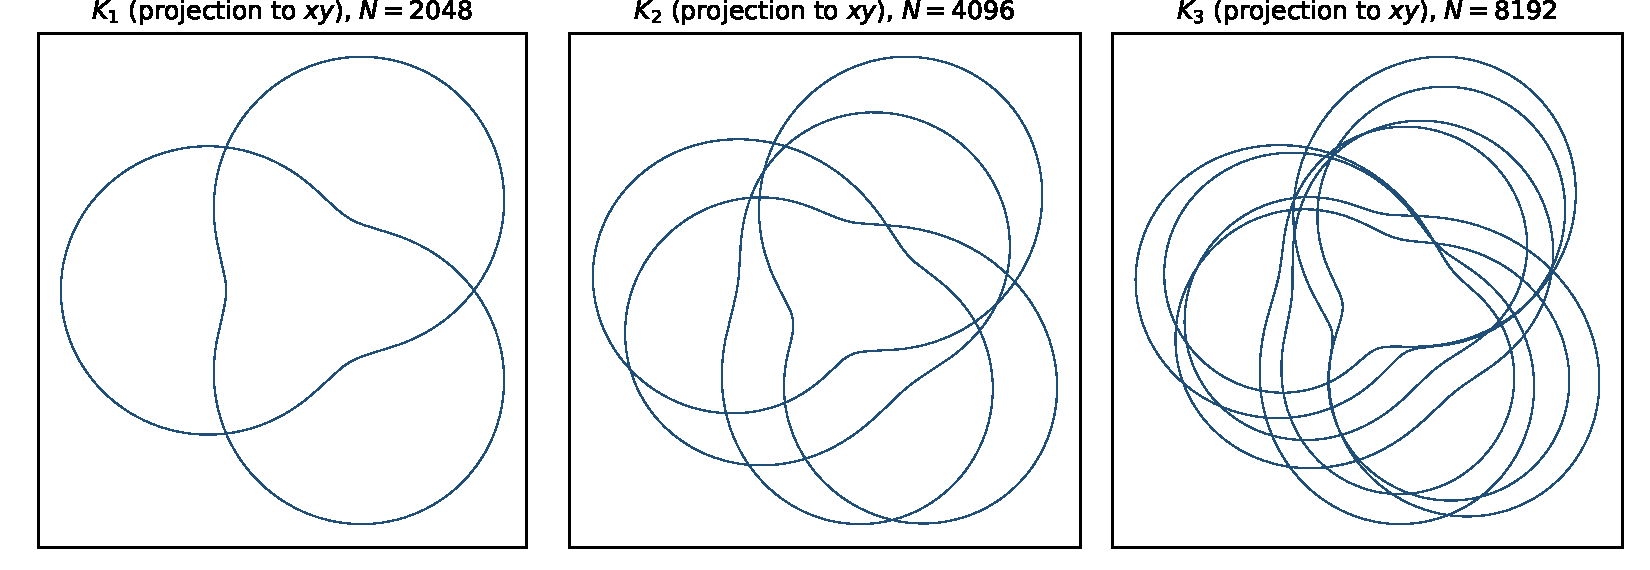
\includegraphics[width=\linewidth]{../figures/fig_curves.pdf}
\caption{Projections to the $xy$-plane of $K_1,K_2,K_3$ for $(2,3)$, $f=0.5$.}\label{fig:curves}
\end{minipage}\hfill
\begin{minipage}[t]{0.38\textwidth}\centering
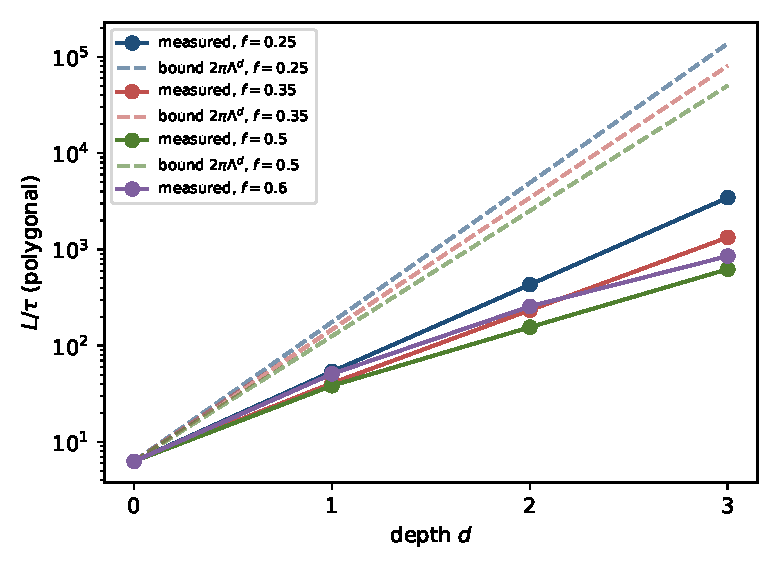
\includegraphics[width=\linewidth]{../figures/fig_rop.pdf}
\caption{Polygonal $L/\tau$ against depth for the default family (solid) and the conditional bound $2\pi\Lambda^d$ with $c=1/2$ (dashed, $f\le1/2$).}\label{fig:rop}
\end{minipage}
\end{figure}

\section{Claims and their status}\label{sec:claims}

\begin{center}\footnotesize
\begin{tabular}{@{}p{0.64\textwidth}p{0.32\textwidth}@{}}\toprule
Claim & Status\\\midrule
$K_d$ is embedded, smooth and regular when $r_d<\thick(K_{d-1})$ (Lemma~\ref{lem:embed}). & proved here\\
The closed Bishop frame has $\Lk=\Wr-\alpha/2\pi$; $K_d$ is the $(p,q+pn)$-cable of $K_{d-1}$ (Lemma~\ref{lem:frame}). & proved here from classical results\\
$pL(K_{d-1})(1-r\kappa_{\max})\le L(K_d)\le pL(K_{d-1})(1+r\kappa_{\max})+r(2\pi q+p|\alpha|)$ (Lemma~\ref{lem:length}). & proved here\\
$\thick(K_d)\le r_d$ and $\Rop(K_d)\ge L(K_d)/r_d\ge2\pi(p(1-f)/f)^d$ for $p=2$ (Prop.~\ref{prop:upper}). & proved here (lower bound internal to the family)\\
Same-disc pairs at distance $\ge2r\sin(\pi/p)$; far pairs at distance $\ge2(\tau-r)$ (Prop.~\ref{prop:partial}). & proved here\\
Different-strand pairs at distance $\ge\min(2(\tau-r),2c_1r)$, $c_1\ge\HcConeBase$ in the $(2,3)$ family, $f\le1/2$, all $d$ (Lemma~\ref{lem:Hc1}). & proved here\\
$\minRad(K_d)\ge1/\bar\kappa_d$ and same-strand doubly critical pairs at distance $\ge\min(2(\tau-r),2c_0r)$ (Props.~\ref{prop:Hccurv}--\ref{prop:Hcsame}). & proved here under $(\mathrm H_3)$; unconditional at $d=1$\\
$\thick(K_d)\ge\min(\tau-r,cr)$ with $c=1/2$, $p=2$, $f\le0.35$, $d\le3$ (Thm.~\ref{thm:Hc}). & proved at $d=1$; at $d=2,3$ under $(\mathrm H_3)$ with measured constants\\
No $c>0$ depending only on $(p,q,f)$ works for an arbitrary base $K$ (Remark~\ref{rem:Hcfalse}). & proved here\\
$(\mathrm H_c)$ for the family with $c=1/2$: same-strand case at $f=1/2$, uniformity in $d$. & not proved; verified numerically in $\HypLevels$ levels, margin $\ge\HypMinTauOverRho$ ($c=1$ fails in $\HypFailOne$ of $\HypLevelsAll$ levels)\\
$\Rop(K_d)\le2\pi\Lambda^d$, $\Lambda=A/\gamma$ (Cor.~\ref{cor:rec}). & proved conditional on $(\mathrm H_c)$ for the family\\
Explicit polygons with $L/\tau=\RopHalfOne,\RopHalfTwo,\RopHalfThree$ at $d=1,2,3$ ($f=0.5$), stable to $\ConvMaxRelRop\%$. & computationally verified (polygonal proxy, not certified smooth thickness)\\
Knot type of $K_2$ changes between $f=0.35$ and $f=0.5$ (writhe of $K_1$ crosses $3.5$ at $r_1^\ast=\WrCrossRstar$). & computationally verified ($\Wr(K_1)$ stable to $10^{-4}$), consequence of Lemma~\ref{lem:frame}\\
$\Rop\ge c_0\Cr^{3/4}$; existence and regularity of tight knots. & literature \cite{BuckSimon1999,CKS2002}\\
$\thick(K_d)=r_d$ for small $f$ (Conj.~\ref{conj}); then $\Rop_d/\Rop_{d-1}\to p/f$. & conjectural; the rate is a consequence, not a new constant\\
Curve-shortening lowers the polygonal $L/\tau$ of $K_1$ by $\ShrinkPctOne\%$ and raises that of $K_2$. & uncertified numerical probe; negative at depth two\\
Stationarity or optimality of any $K_d$; a recursive flow law for tight recursive knots. & not claimed\\
\bottomrule\end{tabular}
\end{center}

\section{Limitations and next steps}

\emph{Limitations.} (1) The thickness lower bound is fully proved only for different-strand pairs ($p=2$); the curvature of $K_d$ and the same-strand pairs need $(\mathrm H_3)$, whose constants are measured on the polygons for $d\ge2$ and whose uniformity in $d$ is open; at $f=1/2$ the same-strand constant $c_0$ falls short of $1/2$. (2) The polygonal $\tau$ of \eqref{eq:tau} uses vertex pairs and a local-minimum test; agreement with $\tau_{pt}$ to $\PtMaxRel\%$, the segment--segment check of Section~\ref{sec:poly} and stability under doubling of $N$ are evidence, not certification, which would require interval arithmetic on a $C^{1,1}$ interpolant. (3) $r_d$ is a fixed fraction of the measured thickness; nothing is optimised, and the family (pattern angle linear in $t$, phase $\varphi_d=0$) is one of many. (4) The conditional bound $2\pi\Lambda^d$ and the measured chain use different $r_d$. (5) Writhe and holonomy are midpoint-rule sums, accurate to $10^{-4}$ at depth one but only to $\WrDiffMax$ at depth three of $(3,2)$; the frame linking number for $f=0.5$ is decided by a margin of $0.02$. (6) The only lower bound specific to the family is Proposition~\ref{prop:upper}; the knot-type lower bounds need $\Cr(K_d)$, which is not known. (7) The constants of Theorem~\ref{thm:Hc} other than $c_1(\frac12,\frac23)\ge\frac12$ are infima of explicit functions evaluated on grids with an estimated Lipschitz correction, not with interval arithmetic.

\emph{Next steps.} (1) At $d=1$ the uncovered case is an explicit, certifiable computation: the minimal distance between the strands of $T(p,q)$ on the torus of radii $(1,r)$ as a function of $r$ (the critical pair at $f=1/2$ is the pair across the hole, not a local helix pair); for the same-strand case at $f=1/2$ and $d\ge1$, use the exact expression of Proposition~\ref{prop:Hccurv} for $|K_d'\times K_d''|$ with the angle $\psi$ kept, instead of $\kappa_\perp^2+\kappa_W^2=\kappa^2$, to sharpen $\bar\kappa_d$ away from the inner side of the tube; and bound $V_1$, $K_1$ of $K_d$ in terms of those of $K_{d-1}$ to make $(\mathrm H_3)$ uniform in $d$. (2) Replace the polygonal proxy by a certified computation (interval arithmetic on $\minRad$ and $\dcsd$ of a piecewise-circular interpolant) and the midpoint writhe by the exact polygonal writhe. (3) Replace the curve-shortening probe by a constrained length minimisation at fixed $\tau\ge1$ with a certified knot-type check, for $d=1,2$. (4) Optimise $f_d$ per depth and the pattern angle in arclength rather than in $t$. (5) Compute the crossing numbers of the specific cables identified in Lemma~\ref{lem:frame} where known, to attach a Buck--Simon lower bound to each explicit configuration.

\appendix
\section{Reproducibility and protocol}\label{app:repro}

{\sloppy
\emph{Protocol.} \texttt{experiments/recursive\_knots.py} builds the polygon $K_0$ with $N_0$ vertices, computes the closed Bishop frame by discrete parallel transport (rotation taking $T_i$ to $T_{i+1}$, Rodrigues formula; initial normal orthogonal to $T_0$; holonomy measured as the signed angle between the transported and the initial normal, removed by the twist $-\alpha i/N$) and produces $K_d$ with $p_dN_{d-1}$ vertices by \eqref{eq:Kd} evaluated at the vertices (no interpolation; the parameter $t$ is the vertex index). At each depth it measures $L$, $\minRad$, $\dcsd$, $\tau$, $\tau_{pt}$, $\Rop$, the writhe, the holonomy and $\Lk=\operatorname{rint}(\Wr K_{d-1}-\alpha_d/2\pi)$ with its residual, and sets $r_{d+1}=f\,\tau(K_d)$. Grid: $(p,q)=(2,3)$ with $f\in\{0.25,0.35,0.5,0.6\}$, and $(3,2)$, $(2,5)$ with $f=0.5$; depths $1$--$3$; two resolutions, $N_0\in\{\NZeroCoarse,\NZeroFine\}$ ($\{\NZeroCoarseB,\NZeroFineB\}$ for $(3,2)$, whose depth-3 polygon has $27N_0$ vertices). The value $f=0.6$ lies outside the hypothesis $r\le\tau/2$ and is included only as a numerical probe. The computation is deterministic (seed \MetaSeed{} recorded for bookkeeping only); the reference run took $\MetaSeconds$\,s of wall-clock time ($\MetaMinutes$ minutes) on shared cores with Python \MetaPython{} and NumPy \MetaNumpy. \texttt{experiments/aux\_checks.py} computes the critical-pair geometry at depth one, the writhe crossing $r_1^\ast$ and the segment--segment check (\texttt{results/aux\_checks.json}); \texttt{theory/check\_Hc.py} evaluates the constants of Theorem~\ref{thm:Hc} on the polygons and checks every intermediate inequality of Lemma~\ref{lem:Hc1} on all local pairs (\texttt{theory/check\_Hc\_output.txt}, \texttt{check\_Hc\_summary.json}). \texttt{python3 experiments/make\_numbers.py} writes \texttt{manuscript/numbers.tex} and the table body from these JSON files, and \texttt{manuscript/build.sh} runs it and \texttt{latexmk}. Every number in this text is a macro from \texttt{numbers.tex}.\par}

\renewcommand{\bibfont}{\small}
\bibliographystyle{plainnat}
\bibliography{refs}
\end{document}
